\documentclass[review]{elsarticle}

\usepackage{lineno,hyperref}
\usepackage {amsmath}
\usepackage {amssymb}
\usepackage {bm}
\usepackage {bibnames}
\usepackage {graphicx}
\usepackage {graphpap}
\usepackage {longtable}
\usepackage {multirow}
\usepackage {tikz}
\usetikzlibrary {decorations.markings}
\usepackage {varioref}
\usepackage{subcaption}
\setlength{\abovedisplayskip}{3pt}
\setlength{\belowdisplayskip}{3pt}
\modulolinenumbers[5]

\journal{Engineering Fracture Mechanics}

%%%%%%%%%%%%%%%%%%%%%%%
%% Elsevier bibliography styles
%%%%%%%%%%%%%%%%%%%%%%%
%% To change the style, put a % in front of the second line of the current style and
%% remove the % from the second line of the style you would like to use.
%%%%%%%%%%%%%%%%%%%%%%%

%% Numbered
%\bibliographystyle{model1-num-names}

%% Numbered without titles
%\bibliographystyle{model1a-num-names}

%% Harvard
%\bibliographystyle{model2-names.bst}\biboptions{authoryear}

%% Vancouver numbered
%\usepackage{numcompress}\bibliographystyle{model3-num-names}

%% Vancouver name/year
%\usepackage{numcompress}\bibliographystyle{model4-names}\biboptions{authoryear}

%% APA style
%\bibliographystyle{model5-names}\biboptions{authoryear}

%% AMA style
%\usepackage{numcompress}\bibliographystyle{model6-num-names}

%% `Elsevier LaTeX' style
\bibliographystyle{elsarticle-num}
%%%%%%%%%%%%%%%%%%%%%%%

\begin{document}

\begin{frontmatter}

\title{Stress Intensity Factor Surrogate Models Using Genetic Programming Symbolic Regression\tnoteref{mytitlenote}}
% \tnotetext[mytitlenote]{Fully documented templates are available in the elsarticle package on \href{http://www.ctan.org/tex-archive/macros/latex/contrib/elsarticle}{CTAN}.}

% %% Group authors per affiliation:
% \author{Elsevier\fnref{myfootnote}}
% \address{Radarweg 29, Amsterdam}
% \fntext[myfootnote]{Since 1880.}

%% or include affiliations in footnotes:
\author[mymainaddress,mysecondaryaddress]{Elsevier Inc}
\ead[url]{www.elsevier.com}

% \author[mysecondaryaddress]{Global Customer Service\corref{mycorrespondingauthor}}
% \cortext[mycorrespondingauthor]{Corresponding author}
% \ead{support@elsevier.com}

\address[mymainaddress]{1600 John F Kennedy Boulevard, Philadelphia}
\address[mysecondaryaddress]{360 Park Avenue South, New York}

\begin{abstract}
%%% -*-LaTeX-*-
%%% This is the abstract for the thesis.
%%% It is included in the top-level LaTeX file with
%%%
%%%    \preface    {abstract} {Abstract}
%%%
%%% The first argument is the basename of this file, and the
%%% second is the title for this page, which is thus not
%%% included here.
%%%
%%% The text of this file should be about 350 words or less.

Fatigue cracks can be successfully modeled with three-dimensional finite-element (FE) models using FRANC3D. These models are useful in calculating stress intensity factor (SIF) histories that subsequently can be used to integrate crack-growth rate relations and predict the fatigue life of a part. However, when modeling thin structures, it is often computationally desirable to use shell elements. Shell element models can include line-weld elements representing welds connecting the edge of a surface to the face of another surface. The line-weld is modeled with one-dimensional elements that can transmit both translational and rotational forces. Cracks cannot be explicitly modeled in these one-dimensional elements, so we seek alternate methods to simulate fatigue damage in the welds. 

In this work, a surrogate model that relates the translational and rotational loads in the line-weld elements of a C-channel welded to a plate to corresponding SIFs is created with symbolic regression, using the open-source code, Bingo. To train the surrogate model, continuum FE calculations of a typical plate-channel welded connection were conducted for a suite of loading combinations to develop SIF history relationships. Similarly, for the same nominal geometric arrangement and loading conditions, shell and line-weld FE calculations were used to determine the corresponding translational and rotational forces. The resulting model is an interpretable, closed-form, mathematical model that can be used to map the line-weld forces to SIF history and, thus, predict fatigue life. 


\end{abstract}

\end{frontmatter}

%%% -*-LaTeX-*- 

\chapter{Introduction}\label{introduction}

Surface cracks are some of the most common flaws found in welds. These cracks can propagate and render the weld structurally unsound. Stress intensity factors (SIFs) are the driving force of crack growth and are essential in predicting the rate at which a crack grows through a material. Because SIFs are essential for predicting the components' fatigue life, accurate and reliable models are useful to those designing components. Exact solutions exist for calculating SIFs, but only for specific crack types, such as Irwin’s solution to an embedded elliptical crack in an infinite body \cite{tada2000stress}. For the cases that do not have exact solutions, numerical solutions are used in other crack configurations and geometries \cite{wilson1971numerical,lin1999finite,maligno2010three}. In 1971 W.K. Wilson used a boundary collocation method to calculate SIFs. Later, Lin et al. and Maligno et al. used finite element method (FEM) to numerically simulate fatigue crack growth (FCG) after calculating SIFs. Numerical methods are accurate, high fidelity predictors of SIFs but can be computationally expensive. For that reason, surrogate models are often used as low fidelity stand-ins that are much easier to compute.

Raju and Newman found numerical results through FEM for a semi-elliptical surface crack on a surface of a plate loaded in tension \cite{raju1979stress}. The results from this study were then used to create a surrogate model equation. The equations were obtained from systemically curve-fitting the SIFs to polynomials as a function of the crack's geometry \cite{newman1983stress}. Likewise, there are many developed surrogate models that map the stresses of a lower-dimensional model to 3D crack growth \cite{hombal2013surrogate,leser2016probabilistic,leser2017probabilistic}. Hombal et al. use multi-axial load histories in uncracked models to predict the crack growth of complex crack geometry. They use principal component analysis coupled with Gaussian process regression to create this surrogate model. While their method was accurate, it loses interpretability in both parts of the process. Similarly, Leser et al. train surrogate models using Gaussian process regression. We seek an interpretable surrogate model through Symbolic Regression. 

First, data is collected through high fidelity crack growth models. Fatigue cracks can be modeled using 3D continuum elements in a FE mesh using FRANC3D \cite{carter2000automated}. These cracked models are useful in calculating SIF histories that subsequently can be used to integrate crack-growth rate relations and predict the fatigue life of a part \cite{sankararaman2009uncertainty}. 

While SIFs can be calculated using 3D continuum elements, it is often computationally cheaper to use shell elements when modeling thin structures \cite{bathe2006finite}. Shell element models can include 1D elements called a line-weld representing welds connecting the edge of a surface to the face of another surface \cite{osti_1433781}. In this work, fatigue crack growth is predicted; however, representing a crack in these 1D elements is not feasible.  Consequently, we seek a methodology whereby 1D element forces can be used, along with SIFs computed from 3D continuum models, to determine equivalent SIFs for these element topologies. 

Symbolic Regression (SR) is a type of machine learning (ML) analysis used to develop surrogate models from raw data. SR is a subset of genetic programming (GP) inspired by the evolution of genes in nature \cite{banzhaf1998genetic}. SR represents symbolic equations as tree structures and iteratively mutates and crosses over the equations that perform the best on the training data. This regression process differs from classical regression in that the user does not need to input a predetermined functional form of an equation. SR has been used to find free-form natural laws using experimental data, as Schmidt and Lipson were able to show in their work using SR to implicitly find the Hamiltonian description of a double pendulum using only raw, experimental data \cite{schmidt2009distilling}. Wang et al. used raw experimental data of temperature and an order parameter as inputs to a model for system energy \cite{wang2019symbolic}. They found an explicit model for system energy as a function of temperature and the order parameter using SR. Wang et al. sought to find an established theory called Landau free energy expansion. The model found using SR looked very similar to the energy expansion; however, it was missing parts of the equation to which the output was not as sensitive. The similarities of the outputted equation and the expected equation show the importance of domain knowledge while using SR.

To validate the process of using SR as a tool in the creation of SIF equations, we present the proposed methodology on a classical problem. Raju and Newman calculated SIFs along the crack front of a surface crack in a plate loaded in tension \cite{raju1979stress}. From the collected data, they performed a systematic curve fitting by using double series polynomials \cite{newman1983stress} to fit the SIF data to an equation. First, we propose using their very same SIF data in SR to arrive at an equation that fits the data comparatively or better than their original equation. Second, we use newer and more accurate techniques in FE modeling to generate new SIF calculations. We perform SR on the newly generated data to arrive at a new equation.

In the case where SR is used to model cracks for which there is no established law, it has the advantage that a user with domain knowledge can look at the equations found and identify within an equation recognizable patterns, perhaps already known to be laws for similar cracks. This interpretability of SR is its most significant advantage \cite{otte2013safe,McConaghy2011,vladislavleva2008order}. Interpretability is vital in safety-related applications when required to ensure that the model will work outside of the data used to train the model. Often, models used for highly nonlinear data such as those developed using neural networks are mainly black boxes \cite{fujii1996bayesian}. 

Bingo \cite{bingosymbolicregression} is open-source software used for SR. The training data is passed to Bingo, and the evolution of equations is set until the equations reach a predetermined fitness or error. The resulting model is an interpretable, closed-form, mathematical model that can be used to map the line-weld forces to SIF history and, thus, predict fatigue life.

%%% -*-LaTeX-*-

\chapter{Methods}\label{methods}

The purpose of this study is to develop an interpretable machine learning (ML)
model to efficiently compute stress intensity factors (SIFs) from stresses in
1D line weld elements given user-defined initial crack sizes.  The SR model acts
as a low-fidelity surrogate model, mapping line-weld element stresses within a
structural-element model to the SIFs computed from a crack inserted into a
matching solid-element model. This process ensures that engineering
frameworks can utilize highly efficient line weld elements but
still model higher-fidelity 3D crack growth estimates.  A high-level workflow of
the process is shown in Figure \ref{fig:workflow} to illustrate the overall
dataflow. A brief overview of the process is given next, followed by a detailed
discussion of each box in Figure \ref{fig:workflow} in the following
subsections.

As discussed in Section \ref{introduction}, line-weld elements are used in
engineering applications because of their computational efficiency.  However,
because they are 1D, cracks cannot be modeled geometrically, and corresponding
SIFs cannot be computed. For this reason, two models are developed for the same
structural joint. In the first, solid finite elements are used wherein
arbitrary 3D crack surfaces can be geometrically represented and SIFs computed.
In the second, the more efficient structural finite elements, shells and line
welds are used. In this manner, SIFs from the first model (solid elements)
are provided for the second model (structural elements) with matching boundary
conditions and stress states.  

To ensure an adequate match between the solid- and structural-element models,
limits on the applied BCs are determined (box 1), discussed in Section
\ref{fem}.  Next, a sensitivity analysis is performed to provide an initial
guideline for the variation of BCs that must be applied to generate adequate
training data for the ML model (box 2).  At this point, crack growth is
simulated in the solid-element model using Abaqus and FRANC3D to generate the training
data for the applied BCs, crack size, and resulting SIFs (box 3).  Concurrently,
the shell models with line weld elements are simulated with the same BCs to
generate training data for the line weld element stresses (box 4).  At this
stage, the training features are the line weld stresses and crack sizes, while
the training label is the computed SIFs.  These training data are then provided
to the Bingo software for interpretable ML model generation (box 5).  The output
of this process is a ML model, which takes as inputs the crack size and line weld
stresses and returns a SIF estimate, as would be computed by a 3D solid element
model (box 6).  

There are assumptions we are making to map SIFs from stresses in the line-weld element. We know that as a crack grows, the stresses around the crack redistribute. However, in our model, the local stresses in the line-weld are constant for each combination of BCs. Therefore our model assumes negligible stress redistribution as the crack evolves.

\section{Finite Element Models} \label{fem}

The geometry shown in Figure \ref{fig:abaqus_model} represents a C-channel
welded to a plate. The weld is 3 mm thick and creates a gap of 0.05 mm between
the web of the C-channel and the plate. The C-channel is idealized as a constant
thickness. The channel, plate, and weld are treated as one material, and the weld
is idealized as having no heat-affected zone. As discussed above, a
solid-element model of this geometry was generated to compute SIFs for arbitrary
3D cracks initiating at the weld, while the engineering analyses are expected to
utilize a shell-element model of this geometry.  Consequently, to acquire
representative SIFs for the shell-element model, a mapping between the shell and
solid models based on a stress resultant is required.  This ensures that
the SIFs acquired from the solid model match the stress state of the shell model
being analyzed.  Therefore, to enable this mapping, the first task was to develop
matching shell- and solid-element models. 

FRANC3D uses quarter-point wedge elements along the crack front, and the
remaining elements throughout the volume are quadratic tetrahedral elements. For
this reason, quadratic tetrahedral elements were used in the solid-element
model, which is remeshed during crack growth using FRANC3D. The solid-element
model contains approximately 1e6 quadratic tetrahedral elements.  This number of
elements was found to be more than sufficient after a convergence study on
maximum principal stresses on the weld surface. The higher number of elements
was used because smaller elements were needed to facilitate crack insertion on
the weld surface.  

To be more computationally efficient, Franc3D allows one to subdivide a model to
operate more efficiently on a smaller region. This allows for the remeshing to
happen faster and results in fewer elements in the global model. A cube of
side length 12.7 mm from the weld region is extracted with a finer mesh to be
subject to crack insertion and growth. Moreover, this cube is focused at
mid-span of the weld and aligned with the line-weld element in the shell element
model that will provide local stress-resultants. Within this partition is a
smaller partition with an even finer mesh to allow for a 0.05 mm crack to be
inserted into the mesh by FRANC3D.

The shell-element model contains shell elements and line-weld elements. The
length and width of the plate and C-channel are the same as in the 3D model.
The C-channel connects to the plate with a set of 1D line-weld elements to
manage a contact relationship between edges of the C-channel shell mesh and
surfaces of an adjacent plate shell mesh. Line-weld elements consist of a block
of truss elements, and a side set made up of shell elements. Line welds have 4
degrees of freedom: r, s, t, and moment-about r denoted l. r represents shear on
the surface, in the direction of the weld, s represents shear on the surface,
normal to the weld, and t represents tearing away from the surface. These local
coordinates are illustrated in Figure \ref{fig:local_coords}. The shell elements
model is simulated using Sandia’s SIERRA Mechanics software \cite{osti_1433781}
because of its ability to model line-weld elements.

Displacement BCs were applied to the shell and solid FE models.  The BCs
exercise each of the r, s, t, and l deformation modes.  An initial study was
completed to adjust the maximum value of each applied BC such that there was not
one mode that dominated the response of the model.  The numbering of the
surfaces is illustrated in Figure \ref{fig:surface_nums}. For r-loading,
surfaces 6 and 60 are displaced in the positive z-direction. For s-loading,
surface three is displaced in the positive x-direction. For t-loading, surfaces
4 and 40 and displaced in the positive y-direction. Finally, for l-loading, surface
four is displaced in both the positive and negative x-direction. 

The shell-element model utilized here inherently uses nonlinear geometry. However, the solid model did not include nonlinear geometry to save a substantial amount of computing time. Consequently, with increased applied BC values, the
results of the shell and solid models were observed to diverge.  It was decided
that, to limit this discrepancy, the applied BC values would be limited, such
that a difference of less than 1\% in resultant displacement between the shell
and solid model was observed, see Figure \ref{fig:workflow}.  In some cases, the
applied BC limits were further reduced to ensure that a single applied BC would
not dominate the maximum principal stress response, as discussed in Section
\ref{sensitivity_analysis}.

\subsection{Sensitivity Analysis} \label{sensitivity_analysis}

A sensitivity analysis was conducted to quantify the effect that each applied BC
has on the variability of the stress response in the weld in the FE models. The
sensitivity analysis results are used to determine how to fill the parameter
space during the training data generation step efficiently. For this, a Sobol’
sensitivity analysis was conducted \cite{sobol1990sensitivity}. The Sobol’
method estimates the variance contribution of each parameter and is represented
by the ratio of variance contribution to the total variance of the stress
response. This is referred to as the ``main effect'' of the variable.  Another
index can be found using the Sobol’ sensitivity analysis, which is the
``interaction effect'' and accounts for the impact of model variance due to the
interaction of two parameters.

The sensitivity study is done by first sampling 100 different combinations of
applied BCs using Saltelli’s sampling scheme \cite{saltelli2010variance}, for
which the SALib Python module was used \cite{Herman2017}. SALib takes as inputs
the applied BCs, their ranges, and the desired number of samples to be used in
the sensitivity study.  It then outputs the sampled applied BC values to be
applied. The sampling method is quasi-random and evenly populates the space.

The applied boundary conditions supplied by Saltelli's sampling scheme are
applied to the solid models, which is then analyzed using Abaqus. The dependent
variable of interest is the maximum principal stress at a single point on the
surface of the weld. This is illustrated in Figure \ref{fig:local_mps_point},
showing the local model and the finest mesh and the point at which the maximum
principal stress is calculated. The maximum principal stress was extracted at
the same point in all simulated results to ensure consistency among all cases.

At the end of the sensitivity study, the relative effect that each of the
applied BCs has on the maximum principal stress is known. For each sampled BC,
the applied value during the generation of the simulated training data is then
dependent on its sensitivity. For the BC with the greatest sensitivity, we assign
five applied BC values to be simulated. The global BC with the next largest
effect will have four unique displacements assigned.  The two global BCs with
the smallest effect will have three unique displacements.  The combination of
each of these applied BCs combinations results in 180 unique combinations to be
simulated.  According to Bellera, et al. these 180 combinations will result in a
90\% confidence interval and 10\% margin of error \cite{bellera2007method}. 

Cracks were then inserted and propagated through the solid model using Franc3D
\cite{carter2000automated} for each of the 180 applied BC combinations. The
initial semi-circular surface crack radius was 50 microns, which was determined
to be significantly smaller than the detectable crack size
\cite{christner1988nde} for this structure. The cracks are grown in 10
increments to a depth of 2.4 mm: 80\% of the thickness of the weld. At this
relative crack depth, linear elastic fracture mechanics (LEFM) assumptions break down because unconstrained plasticity would occur in the remaining ligament. Furthermore, in Section \ref{franc3d}, it is shown that ten increments
of crack growth are sufficient to result in converged SIF v.~crack depth
results.  SIFs were computed using the M-Integral method in FRANC3D
\cite{warzynek2005m}. 

\subsection{Data Collection} \label{franc3d}

FRANC3D, a program created by the Cornell Fracture Group, is used to insert and
grow cracks through a finite element model \cite{carter2000automated}.
Specifically, herein, semi-elliptical surface cracks are inserted and propagated
through the weld and in the direction governed by the maximum principal stress.
Upon inserting or growing a crack with FRANC3D, the local region is remeshed to
accommodate the changing topology.  The new mesh that surrounds the crack front
includes three concentric rings of eight elements each. This was chosen because it
has shown to consistently give a converged result for SIFs in surface cracks
\cite{raju1979stress}, including in the models presented herein.  

The size of the crack growth increments must balance efficiency with accuracy.
For this, a convergence study on the step size of the crack extension was conducted
on the pure unidirectional loading conditions.  This convergence study started
each case with a crack of depth 0.05 mm oriented perpendicular to the maximum
principal stress at the location in the weld with the highest maximum principal
stress.  The crack was grown with three different step sizes. One with 20 steps of
0.11 mm, another with ten steps of 0.24 mm, and another with five steps of 0.5 mm.
The percent difference of the SIFs at the depth of the crack was used to
measure convergence of the crack step size. The results of that study are discussed in section \ref{franc_results}. It was found that ten steps of 0.24 mm was sufficiently converged for our purposes.

Concurrently with the previous data collection step, Sandia National
Laboratories’ SIERRA Mechanics software \cite{osti_1433781} is used to simulate
the same 180 combinations of applied BCs on the structural-element model. The
material model used for both the structural- and solid-element FE models is
linear elastic, isotropic steel with a modulus of elasticity of 208 GPa, and
Poisson's ratio of 0.33. A convergence study on the
mesh size of the structural mesh was done, and results compared to the
displacements of the solid model.  From the structural-element simulations,
line-weld element stresses are computed and written to the Sierra output file
for subsequent post-processing.  These stresses, along with the crack depths, a, and the
SIF data generated from the cracked 3D solid element models, are defined as
input features (r, s, t, l, and a) and label ($K_I$). The
values are aligned in a table and inputted into Bingo, a NASA produced,
open-source symbolic regression software \cite{bingosymbolicregression}. 

\subsection{Symbolic Regression} \label{symbolic_regression}

Symbolic regression (SR) is the process of searching the space of real-valued
equations to fit training data. The output of a successful SR is an
interpretable, free-form equation that models the data. It has been used by
Schmidt and Lipson to (re)discover known conservation laws from experimental data of
the positioning of an oscillating double pendulum through time
\cite{schmidt2009distilling}.  Here, we will use SR explicitly. That is to say,
that all input parameters will result in a constant that corresponds
unambiguously to the dependent variable.

Within the SR algorithm, equations are often represented using acyclic graphs,
which have been shown to converge similarly to tree structures but are
computationally more efficient to evaluate \cite{schmidt2007comparison}. The
acyclic graph is illustrated in Figure \ref{fig:agraph} and is stored in the
computer as a list of operations. The largest number of operations in the list
is a user-specified called the stack size. Equations do not always use every
operation in the stack and can be simplified to just the used nodes.
The number of operations in the simplified stack is the complexity of the model.

The SR implementation within Bingo relies on Genetic Programming (GP). GP is the
process by which equations evolve to arrive at a free-form equation that fits
the data. The acyclic graph structure allows for mutation and crossover to
facilitate evolution. Crossover occurs when two acyclic graph individuals create
a new individual when one individual is trimmed at a node. Another portion of
the other individual is randomly attached to the trimmed node. A mutation occurs
when a node in the acyclic graph is changed at random. Both mutation and
crossover events occur with user-defined probabilities.

After evolving one generation, the individuals in the population are compared to
the data to evaluate the fitness, herein measured as the mean absolute error. An
age-fitness evolution strategy is applied too. This means that for a new
individual to survive through to the following generations, it must represent an
improvement of fitness. If a new individual has a similar fitness to that of an
older individual, then the older individual is preferred. Lastly, Bingo allows
for parallel processing of the evolution on multiple cores for faster
convergence. Each core is treated as an island that evolves its own population
of models. At every \textit{n} generations, migration can occur among the
islands, at which point individuals from one island are sent to another island
where they may crossover and mutate.

Because an equation for SIFs in a line-weld element is an usolved problem, we validate our method with a well-studied problem. Raju and Newman \cite{raju1979stress} use systematic curve fitting on their SIF data of a surface crack in a tension-loaded plate. The result of this curve fitting is a closed form equation to fit the data with a mean absolute error of 0.058.

The equation found by Raju and Newman is made up of multiple separate equations that are multiplied together. We decide to follow a similar approach using SR. Equations are found by using Bingo for SR to a set number of generations. If after the set number of generations the equation does not have a lower mean absolute error than the Raju and Newman equation, we use what we refer to as a SR boosting method. 

The boosting method we use for SR is done by fitting a new equation to data normalized by the previous equation's predictions. The resulting output is a number of equations, that when multiplied together, make a better prediction than any single equation on its own. This process is repeated until the addition of more equations does not significantly improve the overall fit of the model.

The overall purpose of this work is to use SR to find an interpretable equation
to act as a surrogate model to map the stresses in a line weld to the SIFs in a
cracked 3-D model. This is done by using the SIFs calculated by Franc3D along
the crack front and the stresses found after analyzing the
structural-elements model as the input training data for Bingo. Explicitly,
the equation should give SIFs as a function of r, s, t, and l stresses as well
as crack size and $\phi$, the parametric angle along the elliptical crack front. 

An essential consideration of SR, and all ML in general, is avoiding over-fitting
the training data. In SR, we have found it useful to limit any consideration of
the produced equations to those with relatively low (reasonable) complexity.
Complexity is a measure of the number of mathematical operations present in the
model. After evolution in SR, many individuals remain with varying complexities
and fitness. These can be plotted as a Pareto front so that we can call out the
equations with the best fitness at each complexity.  Often, the higher
complexity individuals do not significantly improve fitness, as illustrated in
Figure \ref{fig:pareto_front}. This is because the more complex models are over-fitting the training data and not generalizing well. 

The SIF and stress data generated is split into two groups: a train set and
a test set. The train set consists of 80\% of the data and the test set, 20\%.
The data will be split randomly, ensuring that entire load scenarios are
withheld for testing. This ensures that the model doesn't over-fit data that may
be very close to it and will be able to be tested on loading scenarios that it
hasn't seen yet. 

The genetic process for the creation of this model will have 1000 individuals
and a maximum stack size of 64. It will be allowed to evolve for 20,000
generations, or until it reaches convergence, determined as an error below 5\%.
The resulting equations from this evolution will be evaluated by human
interaction, searching for patterns common to SIF equations to find some
interpretability in the model.  The best performing, interpretable equations
will then be evaluated on the test set of data. The equation that performs best
on our test dataset will be our resultant model. 

\begin{figure}
\centering
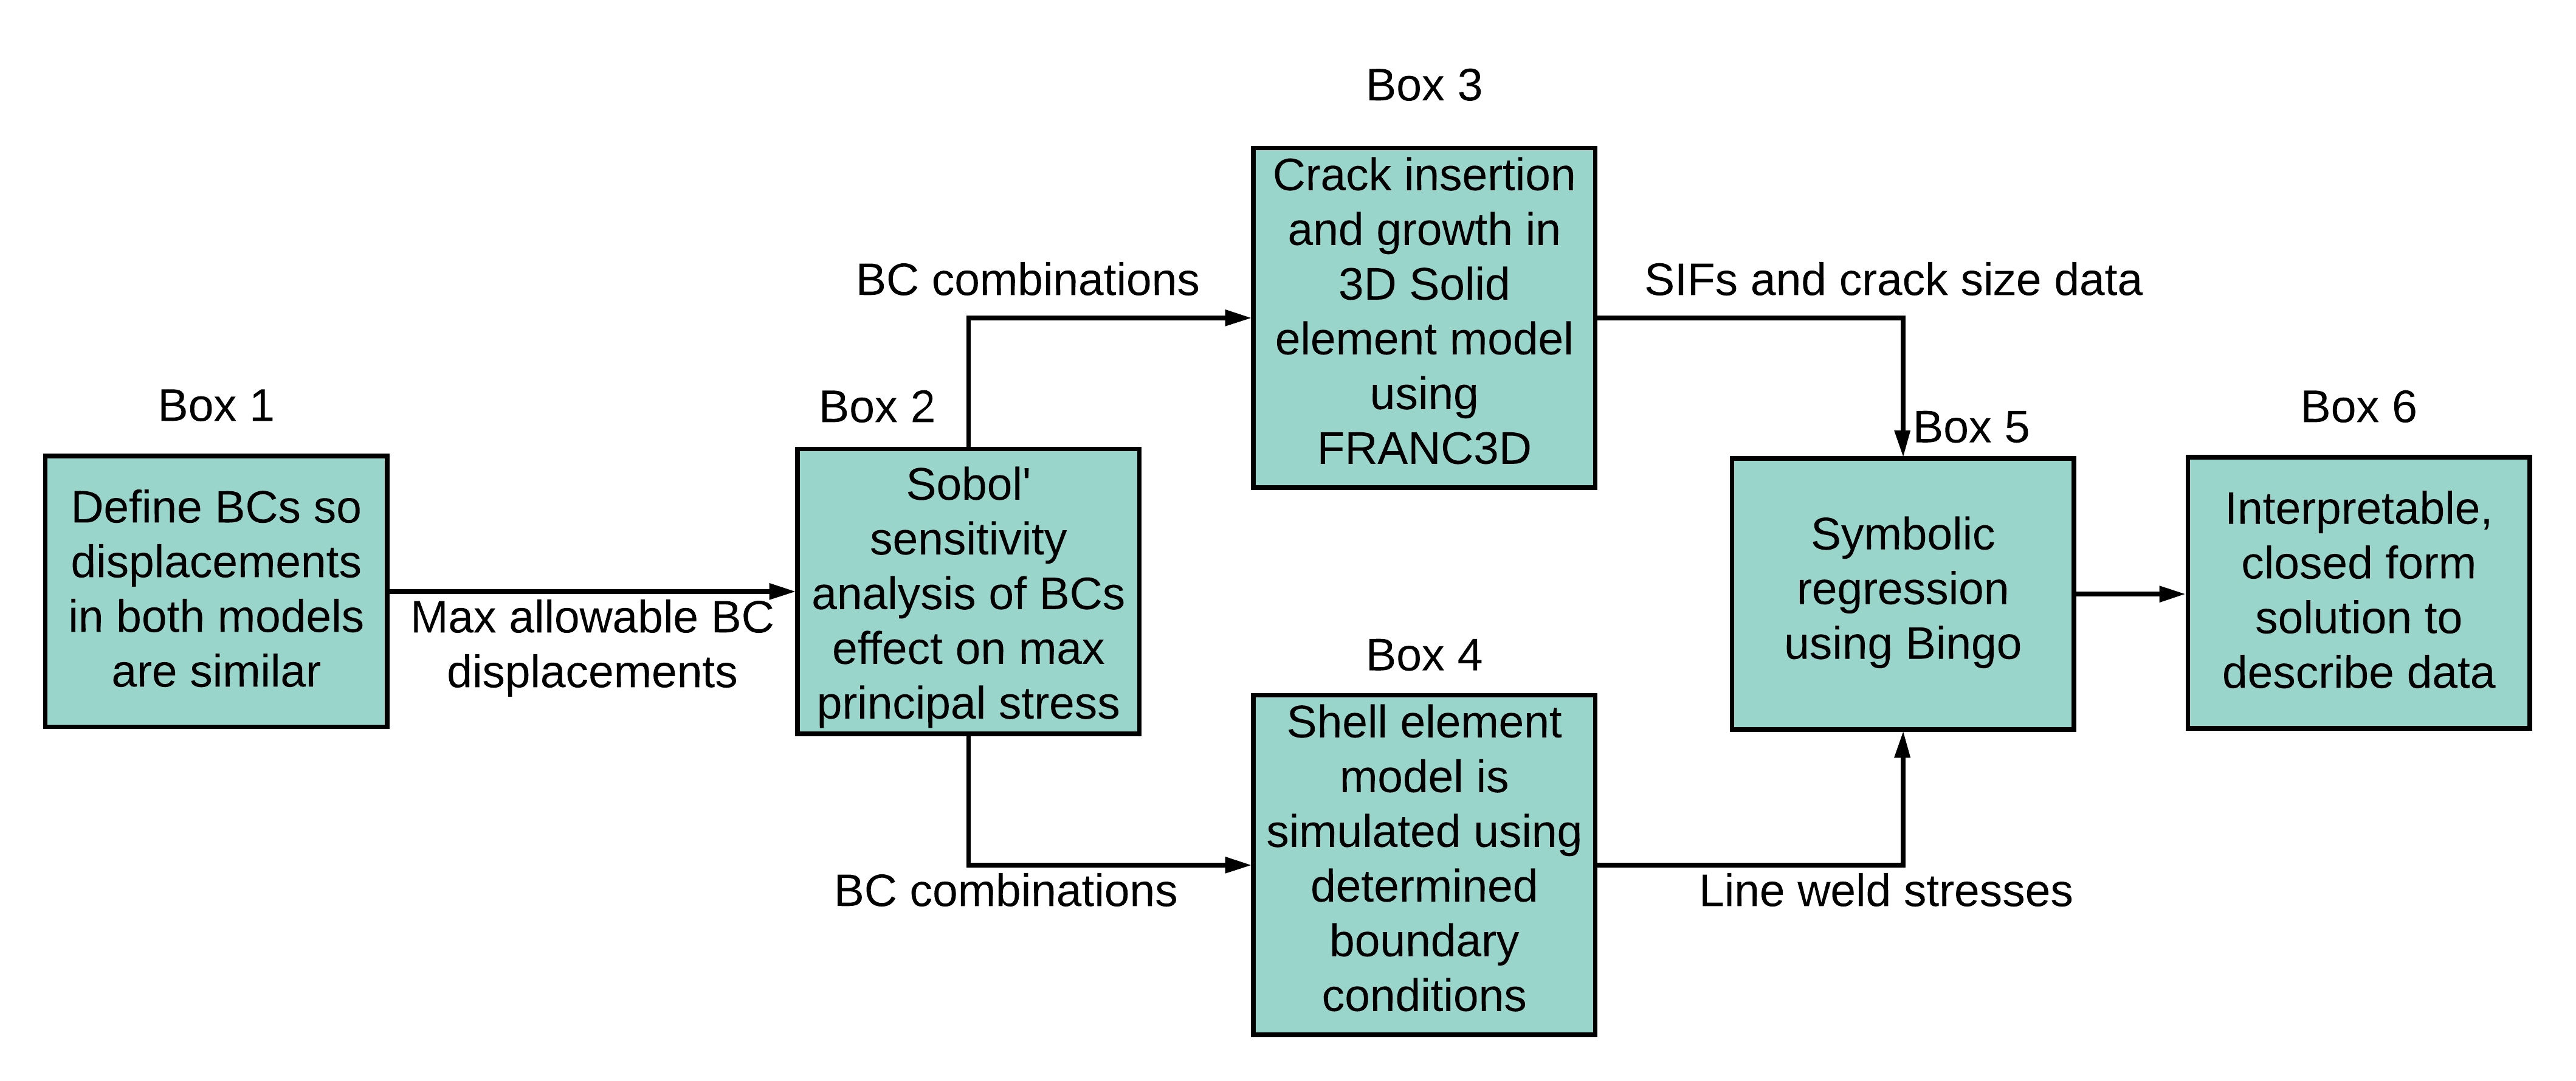
\includegraphics[width=\textwidth,height=\textheight,keepaspectratio]{workflow.png}
\caption{High-level overview of study workflow.}
\label{fig:workflow}
\end{figure}

\begin{figure}[h]
\centering
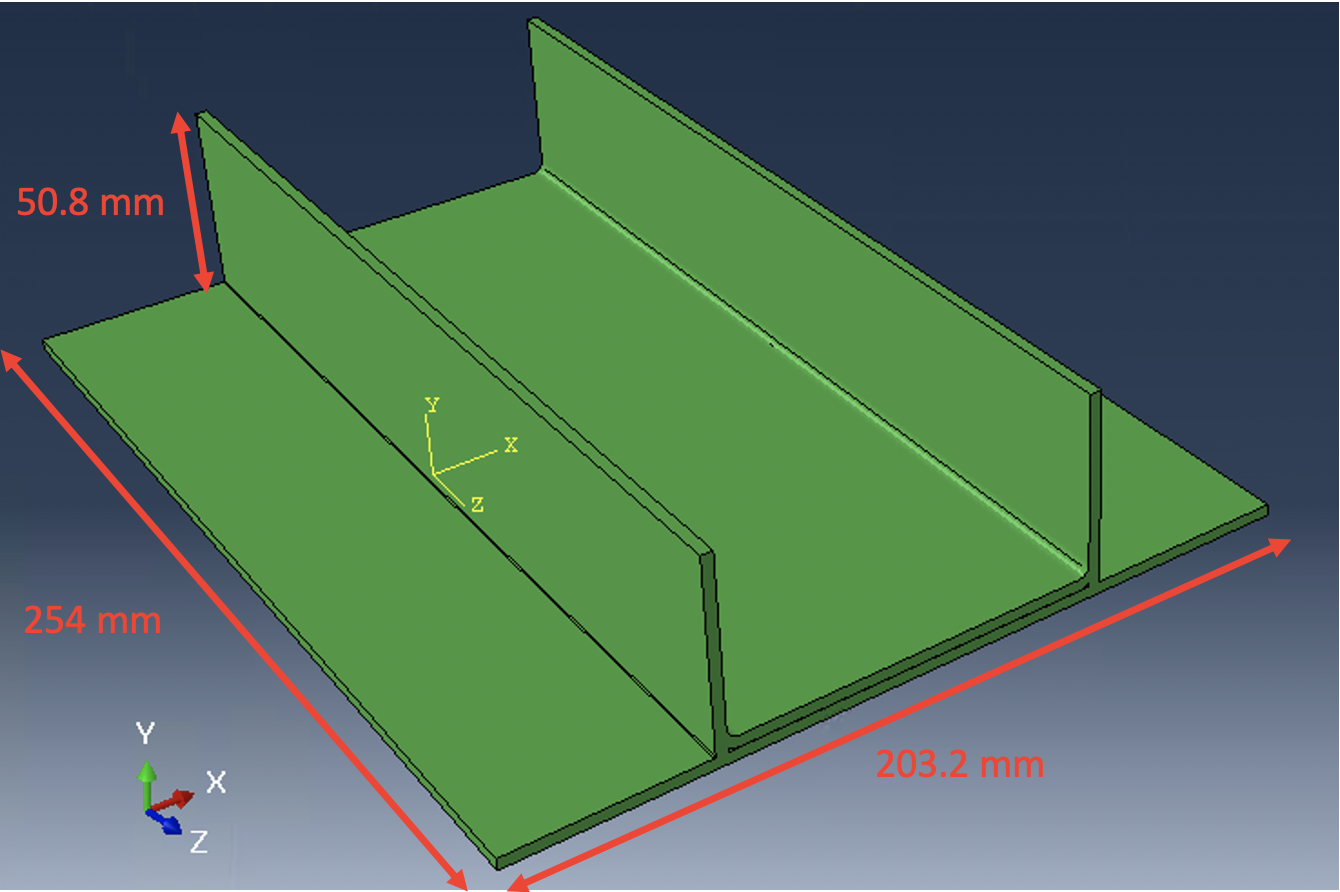
\includegraphics[width=\textwidth,height=\textheight,keepaspectratio]{abaqus_model.png}
\caption{Representation of geometry used to model the C-channel welded to the plate.}
\label{fig:abaqus_model}
\end{figure}

\begin{figure}[h]
\centering
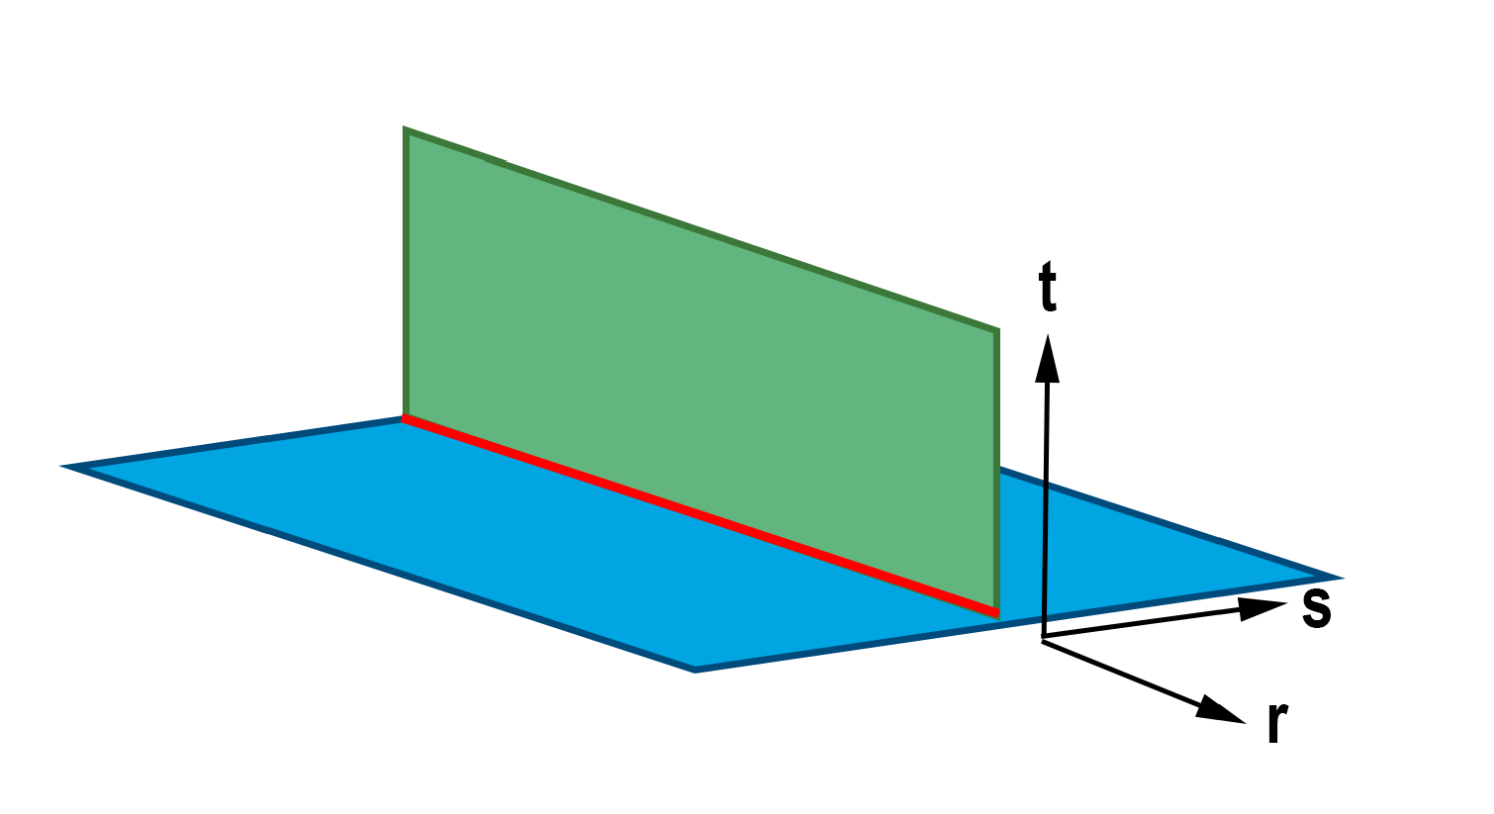
\includegraphics[width=\textwidth,height=\textheight,keepaspectratio]{local_coords.png}
\caption{Illustration of the line-weld local coordinates. The green surface
represents the edge to which the blue surface is welded. The red line represents
the line-weld elements with coordinate axes shown.}
\label{fig:local_coords}
\end{figure}

\begin{figure}[h]
\centering
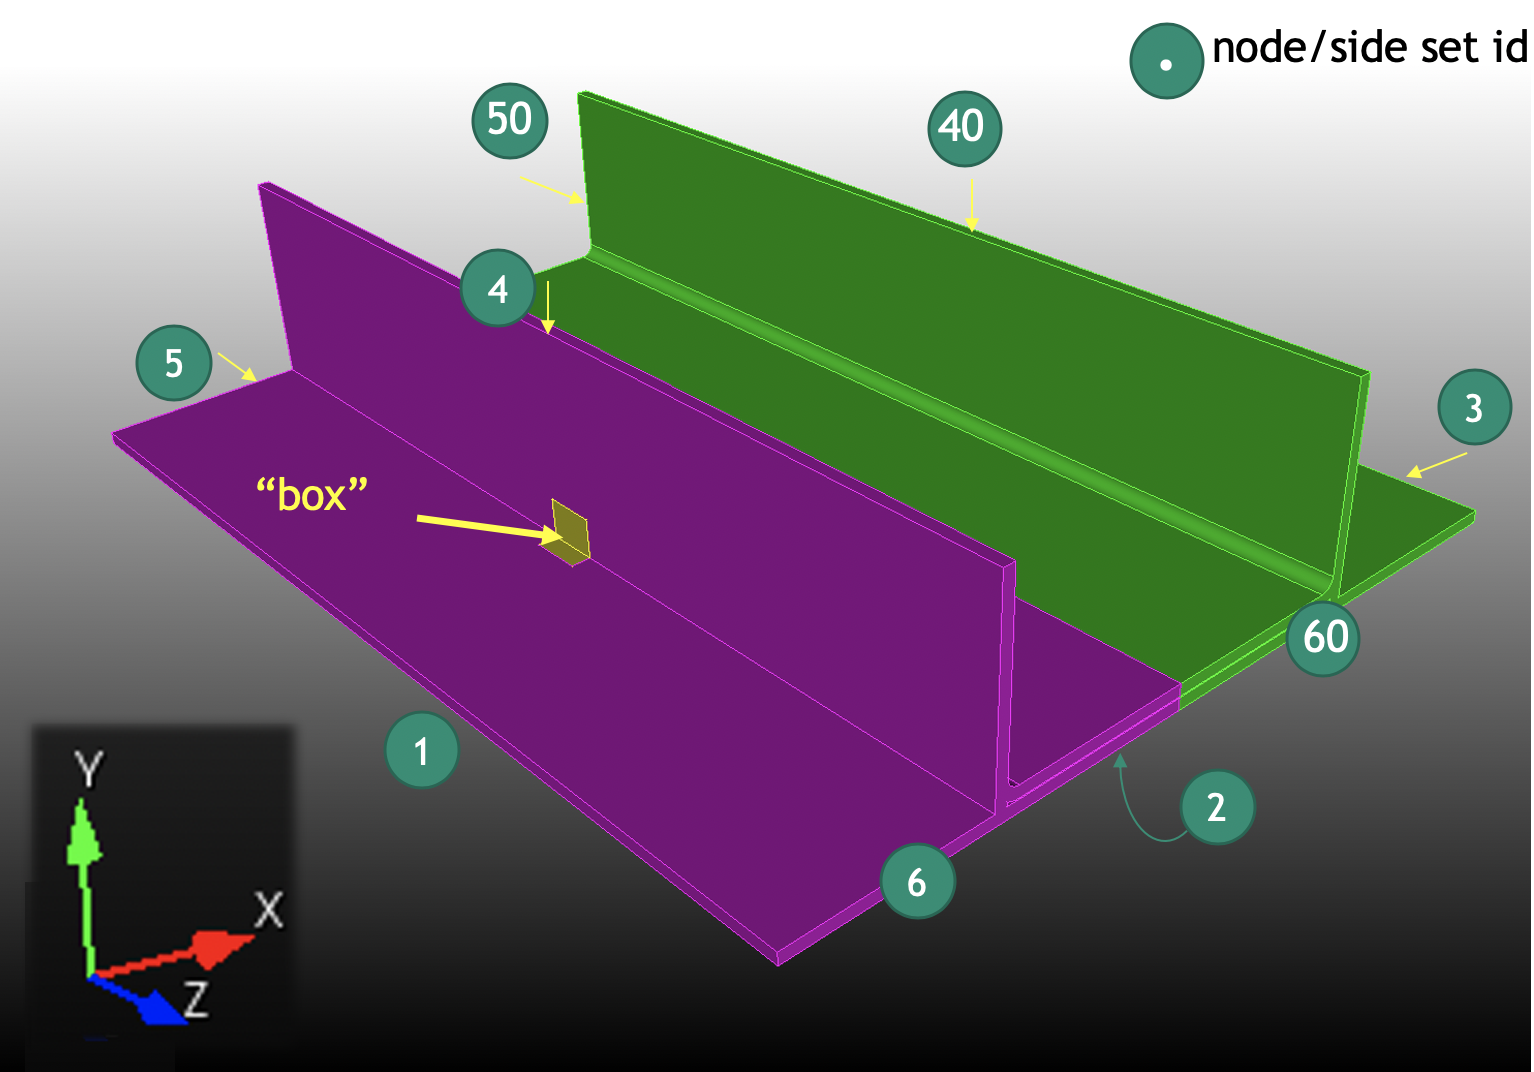
\includegraphics[width=250pt,height=\textheight,keepaspectratio]{surface_numbers.png}
\caption{C-channel welded to a plate with local ``box'' illustrating the local
mesh into which the crack will be inserted. Surface numbers are shown. The
purple and green indicate halves of the model separated by a plane of symmetry.}
\label{fig:surface_nums}
\end{figure}

\begin{figure}[h]
\centering
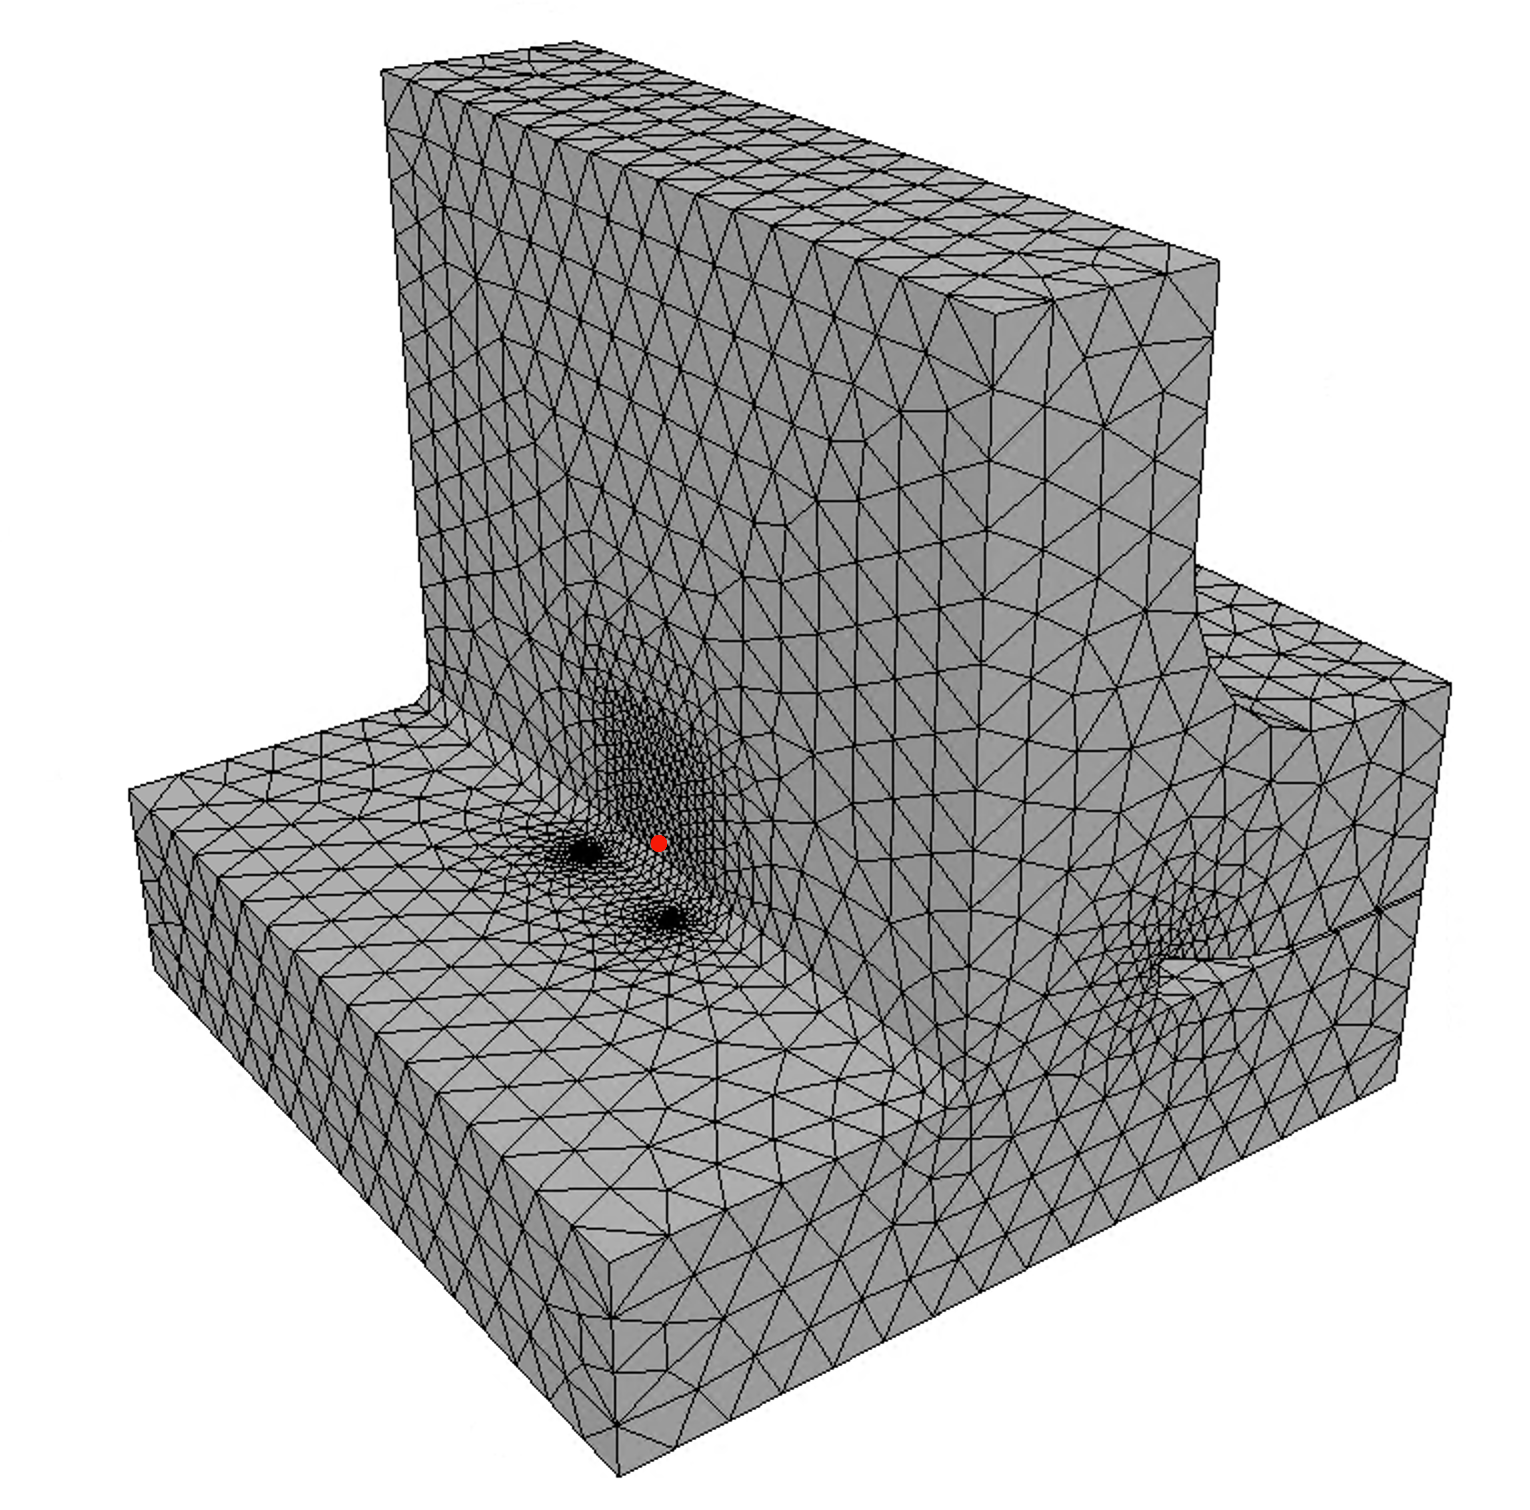
\includegraphics[width=250pt,height=\textheight,keepaspectratio]{local_mps_point.png}
\caption{Local model into which the crack is to be inserted. The maximum principal
stress is calculated at a single point indicated by the red dot. The finer mesh
is shown which facilitates crack insertion.
}
\label{fig:local_mps_point}
\end{figure}

\begin{figure}[h]
\centering
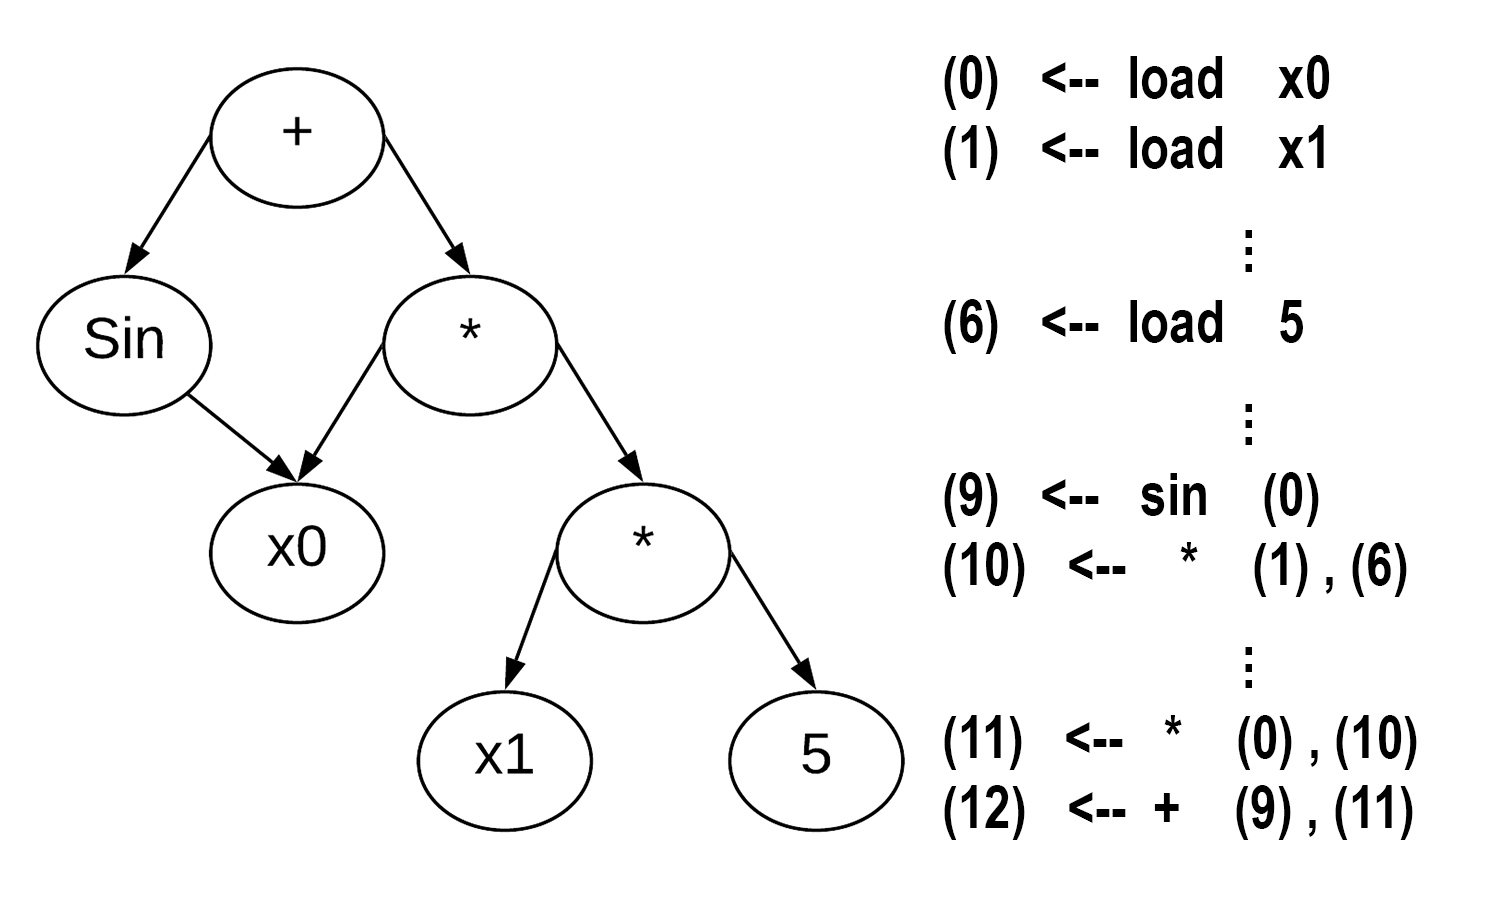
\includegraphics[width=250pt,height=\textheight,keepaspectratio]{agraph.png}
\caption{The equation $f(X) = \sin(x_{0}) + 5*x_{0}*x_{1}$ represented as both a
connected acyclic graph and a list of operations. It's important to note that
the equation is represented without using all nodes in the stack.}
\label{fig:agraph}
\end{figure}

\begin{figure}[h]
\centering
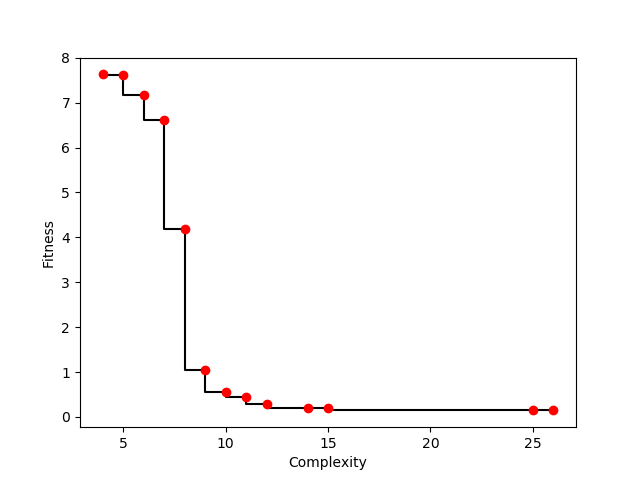
\includegraphics[width=250pt,height=\textheight,keepaspectratio]{pareto_front.png}
\caption{Pareto front of the individuals in a SR population. As complexity
increases, fitness tends to decrease. However, at a certain point, large
increases in complexity do not result in corresponding decreases in error.}
\label{fig:pareto_front}
\end{figure}
%%% -*-LaTeX-*-

\chapter{Results And Discussion}\label{results}
%\section{Finite Element Comparisons}\label{2d_3d_comparison}

To verify the structural-element model, which can only be analyzed with nonlinear geometry, we
compare the displacements of the shell element model to those of the continuum
element model. The displacement BC applied to these models is a 0.01 mm in the
x-direction on surface 3. The first comparison in Figure
\ref{fig:2d_mesh_converge_coarse} shows the two separate models.  The mesh size
of the structural-element model is 12.7 mm. The displacement has been magnified
by 1000 to make clear the deformations. There are apparent disparities between the
displacements of the two models, with the largest being 7\% near the center of
the plate. The mesh size is repeatedly reduced by half until a size of 0.4 mm.
At that mesh size, a percent difference of the displacements falls below 1\%.  

Figure \ref{fig:nl_sload_error} shows the percent error (difference) between the
structural- and 3D solid-element models.  Percent error is computed at 609
points, which are equally spaced out across the model. These points are where the coordinates of the structural element model correspond directly to the coordinates of the 3D solid element model. The distance between the points was approximately the element size of the structural element mesh. The error plotted is the maximum error of the 609 points at
five values of applied x displacement on surface 3.  This BC was chosen for
illustration purposes because it resulted in the largest discrepancies between
the two models.  It is evident that this disparity is due to the eccentricities
in the flanges of the c-channel.

Figure \ref{fig:nl_sload_error} shows a nearly linear relationship between error
and displacement:  the displacement at which error is below 1\% is interpolated
as 0.016 mm. However, to account for possible larger errors when displacements
are combined, the maximum displacement of surface 3 is set at 0.01 mm. A similar
approach is taken for each of the four applied BCs. The results for the maximum allowed
displacement applied to each surface to remain below 1\% error is shown in Table
\ref{tab:max_disps}. 

\section{Sensitivity Analysis}\label{sensitivity_results}

Figure \ref{fig:mps_vs_rstl} shows the relationship between each of the defined
displacement boundary conditions and the maximum principal stress at a single
point at the center of the weld surface.  The results of a Sobol sensitivity
analysis are listed in Table \ref{tab:sobol_indices} as sensitivity indices. We
see that the maximum principal stress is most sensitive to the x-displacement on
surface 4.  The lowest sensitivity index is for x-displacement on surface 3.
However, it has high interaction effects with the other displacement BCs as
evidenced by the larger total effect index, ST. From these results of the sensitivity analysis, to arrive at the 180 different loading conditions we need,
as discussed in section \ref{sensitivity_analysis}, five different displacement
values for the x-displacement on surface 4, four displacement values for the
y-displacement on surfaces 4 and 40, and three different displacement values for
the other two displacement BCs. The 180 different combinations of these BCs will
be our defined BCs for the FRANC3D simulations of crack propagation.

\section{Fracture Analysis}\label{franc_results}

The convergence study discussed in \ref{franc3d} was performed.  Unresolvable errors
occurred within Franc3D in the case where surface 4 is displaced in the
x-direction when the crack growth was too small. Typically, a convergence study
would reduce the size by half at each subsequent step; however, due to the
nature of the re-meshing step in Franc3D, crack size may need to be adjusted to
allow for crack growth.  Therefore, the crack growth sizes for the convergence
study were set at 0.5 mm, 0.24 mm, and 0.15 mm. The SIF calculations were
compared at interpolated points compared to the 0.15 mm step size. Figure
\ref{fig:crack_convergence} shows the percent difference between the 0.15 mm and
the other two crack growth sizes.

The percent difference of SIF at the depth of the 0.24 mm and 0.15 mm crack size
generally stays below 5\% and is a vast improvement from the 0.5 mm crack size.
This difference was deemed small enough to accept and continue. Crack steps
smaller than 0.15 mm were found to increase the remeshing-failure rate within
Franc3D. Also, the computational savings of having fewer crack growth steps was
beneficial for speeding up data collection.

In most cases, cracks were able to grow with a crack growth step size of
0.24 mm. However, during the re-meshing step of Franc3D, parts of the crack front
did not grow far enough past the old crack front in some cases. In these cases,
it was necessary for the crack growth step to be set to a slightly larger size,
up to 0.3 mm.  Other errors encountered using Franc3D were the crack face could
grow to become parallel to the face where the crack front was intended to
intersect. This causes the fitting never to intersect the face and the remeshing
step to fail.  In those cases, we only collected the SIF data up to
the point of failure. However, it should be noted that these cases are also
deemed unlikely to occur in practice and is a direct result of the assumption of
the weld, channel, and plate all being one continuous, homogeneous material.  In
other words, in practice, the crack would be expected to deflect and follow the
weld boundary or heat-affect zone rather than grow through that interface
unperturbed.  Therefore, we concluded that further data in these cases were
practically unnecessary, and no further data was acquired.

Figure \ref{fig:crack_paths} shows different kink angles that defined the crack
increments. For the various cases, the thickness, $t$, is defined as the length the crack would travel to break through an impending surface. The crack
depth, $a$, is defined as the length from the crack insertion point to the deepest point on the crack front along the crack growth path. We see in Figure \ref{fig:crack_paths}, along with the different crack paths, how $a$ and $t$ were defined and how they are dependent on the crack path.

Figure \ref{fig:aKI_pde} shows the density curves of crack length and $K_I$. As noted above, 39\% of the
simulations were not able to grow completely to the desired depth without
failing, which accounts for the lower amount of $a$ values as it gets deeper.
However, due to a majority of simulations that did complete successfully, it was
decided that sufficient data existed for $a$ to perform symbolic regression. 

\section{Symbolic Regression}\label{symbolic_regression}

The model generated from symbolic regression used training data in the form of
$f = \frac{K_I}{\sigma \sqrt{\pi a}}$, where $\sigma$ is the remote stress
idealized as the maximum principal stress at the point of crack insertion and
$a$ is the depth of the crack. The generated model for $f$ is dependent on the
normal vectors of two different planes and the crack geometry $\frac{a}{c}$ and
$\frac{a}{t}$. The first plane, whose normal vector is defined as $\theta_1$ is
the plane created by the initial crack face.  $\theta_2$ is the normal vector to
the plane resulting from a least-squares fit of all the crack front points of
each subsequent crack step. With these two normal vectors, we can
generalize the direction of the maximum principal stress and the direction of
crack growth.  The x-component, y-component, and z-component of $\theta_1$ and
$\theta_2$ are shown as $x, y, z$ and $x_2, y_2, y_3$, respectively

Training on a randomly-selected 80\% of the data set for $f$ with the listed
input vectors after 400k generations of evolution with a stack size of 372
and a population size of 100 resulted in equation \ref{eq:model1}. \begin{equation} \label{eq:model1}
f = \frac{a}{c}\frac{1}{1.5684 * |\frac{a}{c}|^{z_2} + y_2}
\end{equation}This equation,
surprisingly, was not dependent on $\frac{a}{t}$. However, when the results of
the model are subtracted from the actual values of $f$, the model becomes more
correlated with $\frac{a}{t}$. This is illustrated in Figure \ref{fig:f_fsubm1}. 

To improve the model, gradient boosting is implemented.  Gradient boosting, as
described in \cite{friedman2002stochastic} and sequentially fits models to the
residual error of a previous model. This technique results in a more complex,
better fitting model made up of many less complex, weaker models. The final
prediction, defined as $\hat{y}$, is shown in equation
\ref{eq:final_prediction}. Where $M$ is the number of models to be summed, and
$\textbf{x}$ are the inputs to the function $f_m$. Each $f_m$ is found from
training bingo on the residual error of the previous model see equation \ref{eq:f_m}.
\begin{equation} \label{eq:final_prediction}
\hat{y} = \sum_{m=1}^{M} f_m(\textbf{x})
\end{equation}

\begin{equation} \label{eq:f_m}
f_m(\textbf{x}) = y - \sum_{k=1}^{m-1} f_k(\textbf{x})
\end{equation}
Equations found by Bingo are added until the addition of more does not significantly improve the overall fitness of the model.

Because each evolution of Bingo creates a Pareto front of many models, there
exists an optimization problem for which equations to pick that will affect the
residual error and thus the training data on the next training step. The models
are picked greedily by choosing the model which has the lowest mean absolute
error on the test set. The test set is comprised of the remaining 20\% of the
data after selecting the training data.

It is observed that after a certain number of models, the addition of more models
will result in either no improvement or worse fitness
\cite{friedman2001greedy}. To find out how many models can be used to produce
the best results, models are added until the performance of the model on the
test set either converges or becomes worse with the addition of more models. The
performance of the models on the training data and test data is illustrated in
Figure \ref{fig:models_performance}. From these results, the final model is the
sum of equations \ref{eq:f_1},  \ref{eq:f_2}, and \ref{eq:f_3}. As a note,
\begin{equation} \label{eq:f_1}
f_1 = \frac{a}{c}\frac{1}{1.5684 * \frac{a}{c}^{z_2} + y_2}
\end{equation}

\begin{equation} \label{eq:f_2}
f_2 = -0.1657|y|^{\frac{a}{t}}\sqrt{|z|} - 0.1657|y|^{\frac{a}{t}}|||y|^{\frac{a}{t} + |y|^{\frac{a}{t}}}|^{y}|^{0.25} + 0.176
\end{equation}

\begin{equation} \label{eq:f_3}
f_3 = \frac{z\sqrt{|y|}(z_2 - 0.933)}{z(z-1) +1}
\end{equation}
to avoid the possibility of invalid values, Bingo represents everything under a
square root and the bases of an exponent as their absolute value. To not over-saturate the equations with absolute value signs, only those values that can be
negative will be in an absolute value.

Equation \ref{eq:f_2} is not interpretable, at least from a mechanics
perspective, as it has a component of the form $y^y$. Simplification may result
in a more interpretable equation. SR is a great tool to do this kind of simplification.
The training data is created by inputting the variables into the model. This
results in data with zero noise and thus is fairly easy to fit to a SR model.
The resulting Pareto front of equations is tested on the test data, and the model
that results in a similar error as the un-simplified $f_2$ is chosen as the model.
This simplification technique resulted in equation \ref{eq:f_2_simple}. The mean
absolute errors of the summed models on the test data set are shown in Table
\ref{tab:fitnesses}. There is only a 0.6\% difference between the mean absolute
error of $f_1 + f_2$ and $f_1 + f^{'}_{2}$.

As a check for the validity of equations found using SR, a unit analysis is done
as well as defining the domain symbolically. Because all the input variables are
unitless and normalized, each model results in a unitless value. This is
expected because the values used as the label were unitless. A look at input
variables that could cause invalid or infinite values shows us that in $f_1$ we
only get an invalid value when $1.5684*|\frac{a}{c}|^{z_2} = -y_2$. However,
this limitation does not have any immediate interpretable meaning. The functions
$f^{'}_{2}$ and $f_3$ are valid for all input variables.

\begin{equation} \label{eq:f_2_simple}
f^{'}_{2} = -\sqrt{|y|^{\frac{a}{t}}}(0.152\sqrt{|z|} + 0.141) + 0.159
\end{equation}

By only looking at the equations, it is hard to find any interpretable meaning
in a fracture mechanics sense. However, we can gain insights into the equations
by visualizing the surfaces they create in three-dimensional space. Figures
\ref{fig:f1_surf}, \ref{fig:f2_surf}, \ref{fig:f3_surf}, and \ref{fig:f4_surf}
show the raw data plotted with surfaces that represent the summed models. It
represents a three-dimensional slice of the six-dimensional data. We have chosen
$\frac{a}{c}$ and $\frac{a}{t}$ as the input variables to display. These are
typical input variables in fracture mechanics from which we can extract some
physical meaning in the model. We recognize the limitations of viewing a
model with many inputs in only a three-dimensional space.

We see that the first two models go through the general middle of the raw
scattered data. We also see that the summed models that include $f_3$ and $f_4$
begin to predict values that are greater than that of the raw data. Another
important thing to note is the percent error of the prediction and the points. A
physical attribute of the model that we can interpret from the plots is the
steep increase of $f$ as $\frac{a}{t}$ approaches 0.8. This makes physical sense
because we know SIFs increase as the crack grows through a thickness.
\newpage
%% END OF Chapter FIGURES
\begin{figure}
\centering
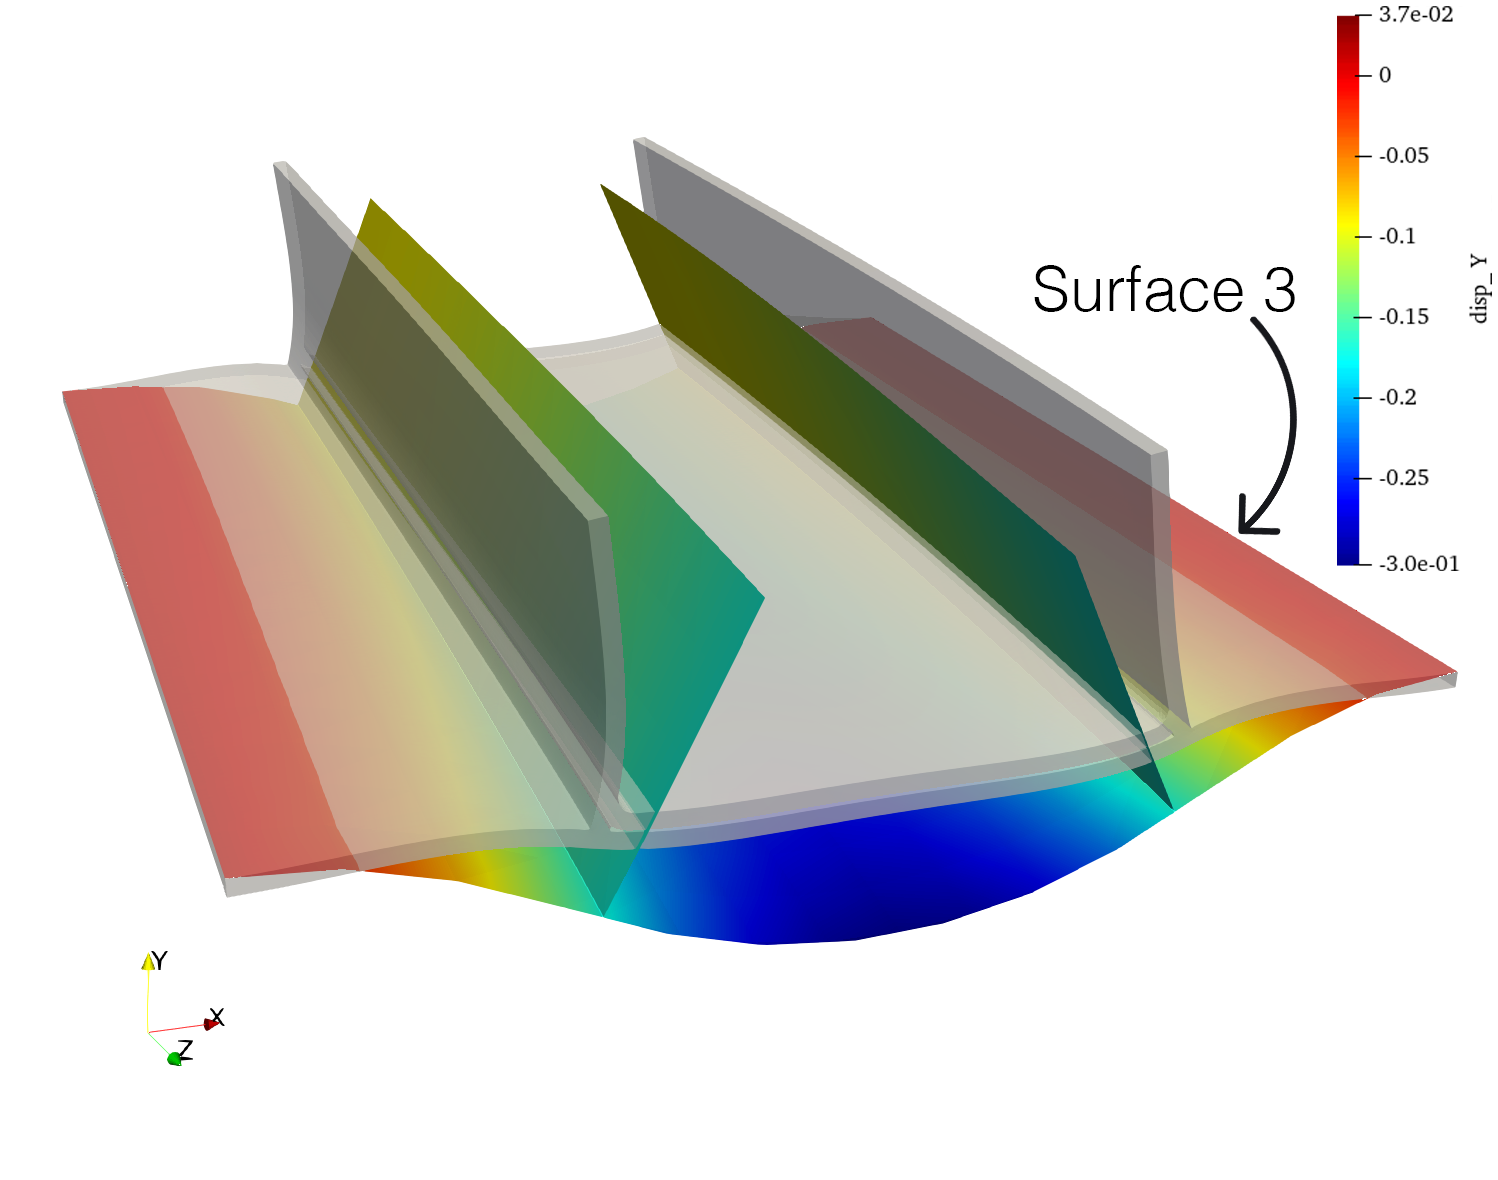
\includegraphics[width=0.65\textwidth,height=\textwidth,keepaspectratio]{2d_mesh_converge_coarse.png}
\caption{Comparison of the structural model and continuum model displacements for the x-displaced surface 3 BC. The mesh size is 12.7 mm. Displacements are magnified 1000x.
}
\label{fig:2d_mesh_converge_coarse}
\end{figure}

\begin{figure}[h!]
\centering
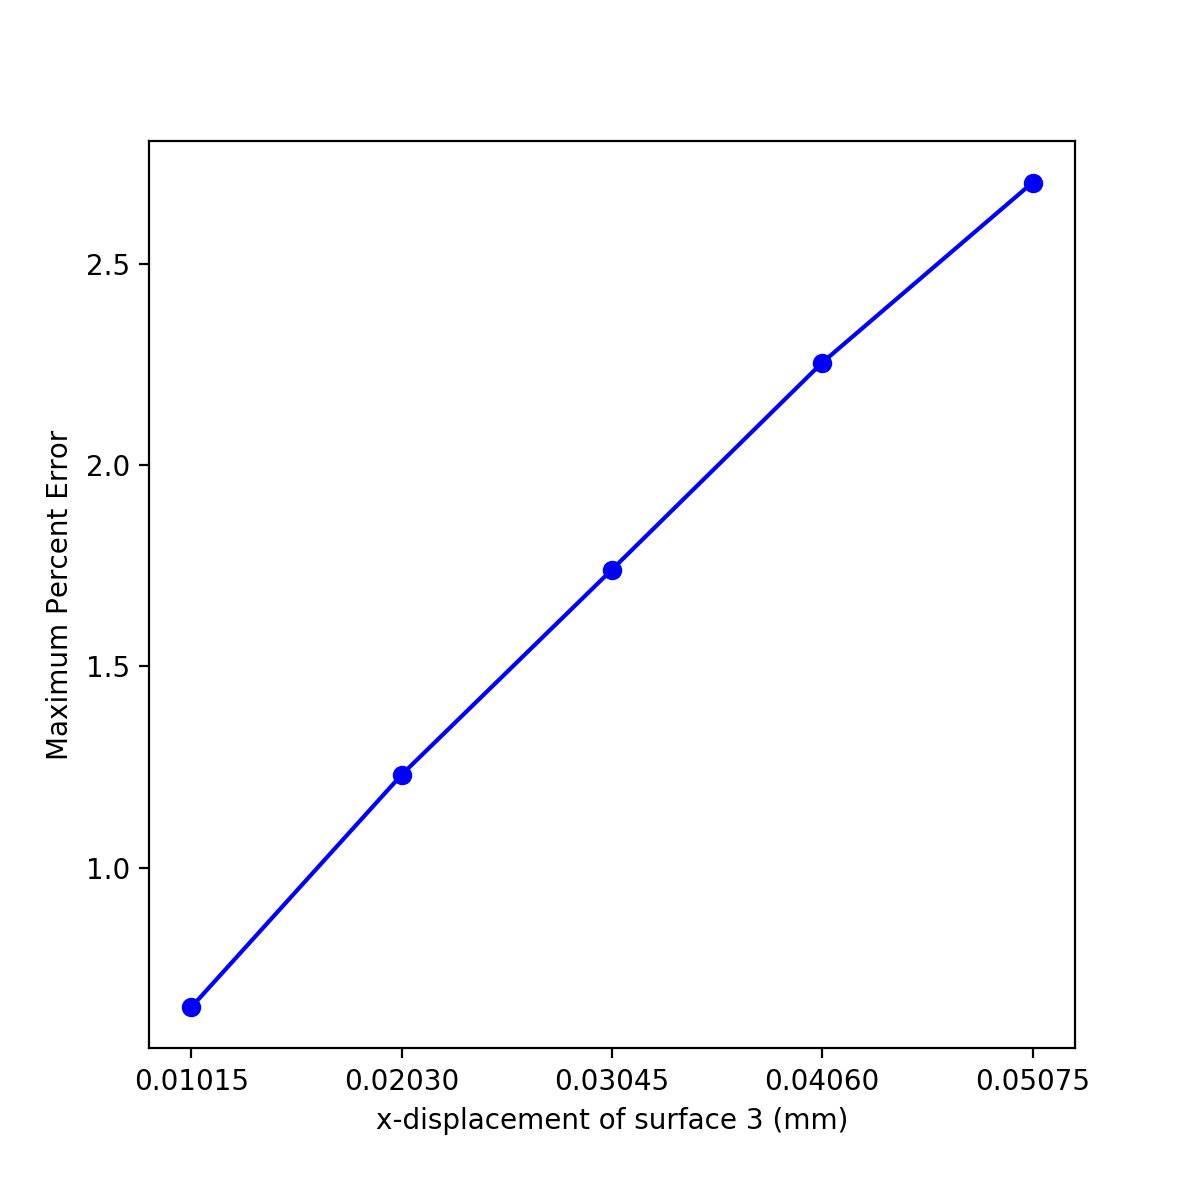
\includegraphics[width=0.65\textheight,height=300pt,keepaspectratio]{nl_sload_error.png}
\caption{The largest percent difference out of 609 points spaced equally across
the model plotted with respect to the applied displacement of surface 3.}
\label{fig:nl_sload_error}
\end{figure}

\begin{figure}[h!]
\centering
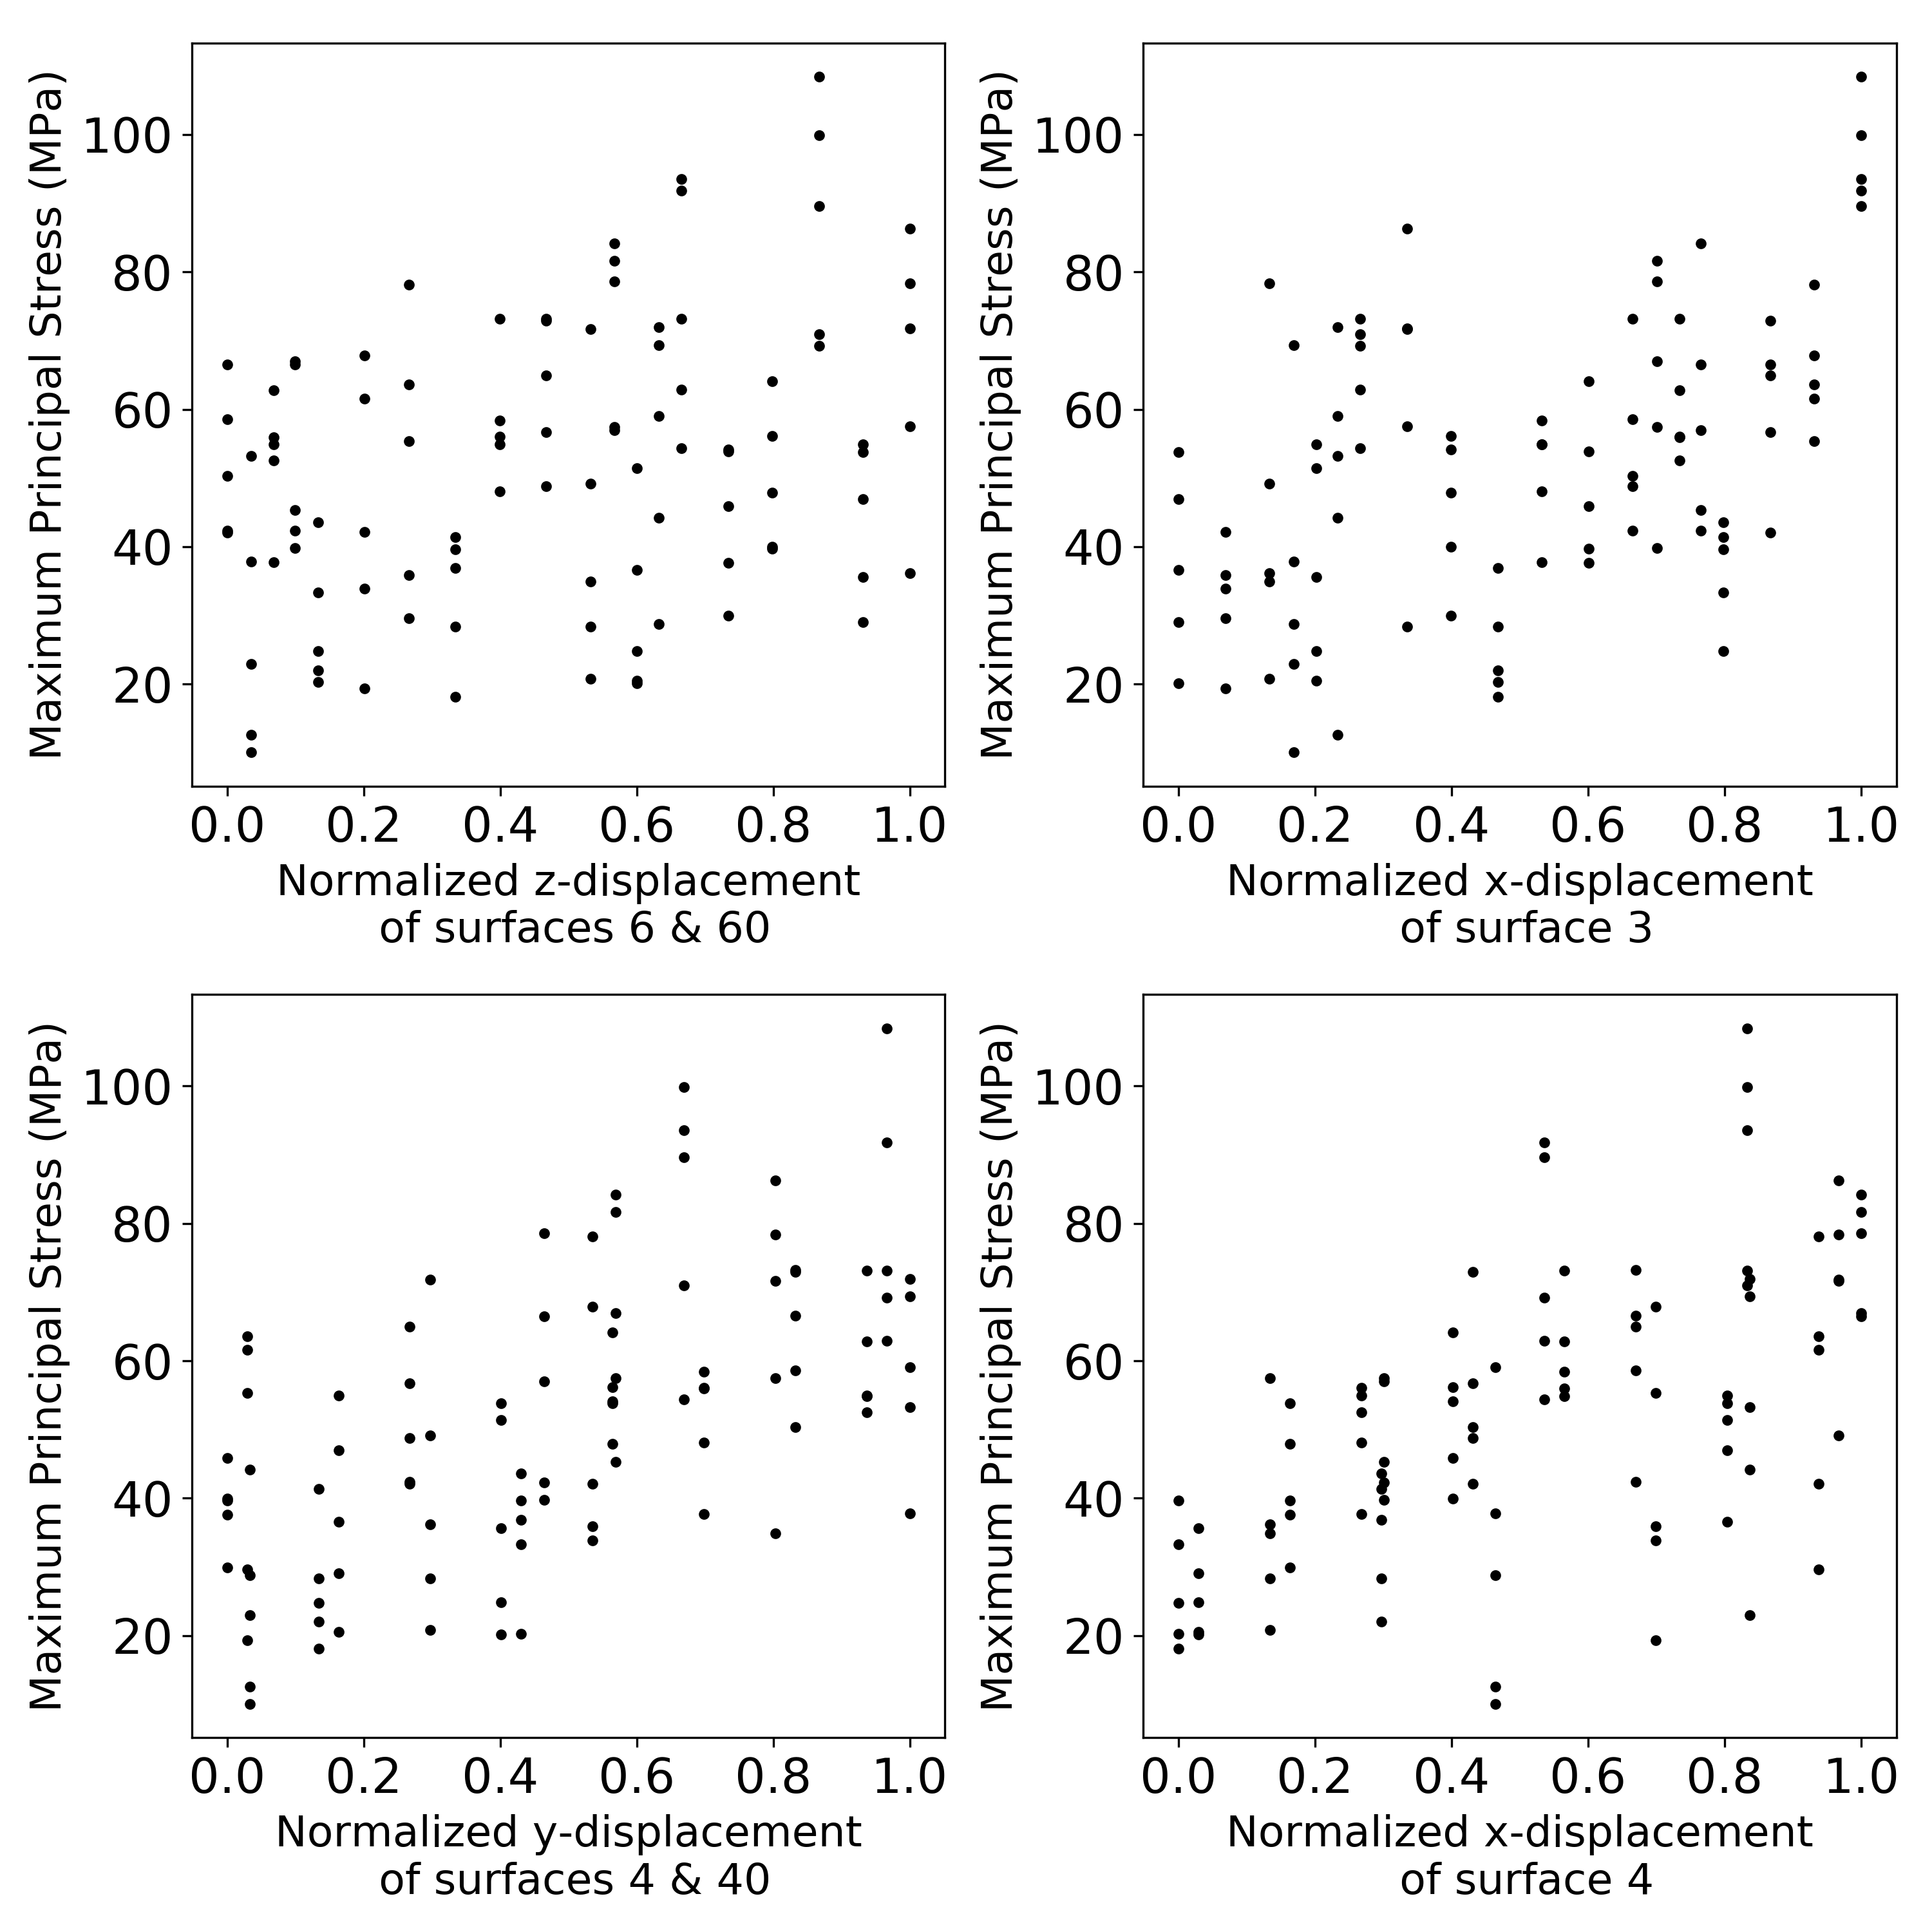
\includegraphics[width=0.6\textwidth,keepaspectratio]{MPS_vs_rstl.png}
\caption{Effects of each boundary condition on the maximum principal stress at a
point in the weld surface center. The point from which the maximum
principal stress is calculated is illustrated in Figure
\ref{fig:local_mps_point}. Displacements are normalized by their maximum applied
displacement BC.
}
\label{fig:mps_vs_rstl}
\end{figure}

\begin{figure}[h!]
\centering
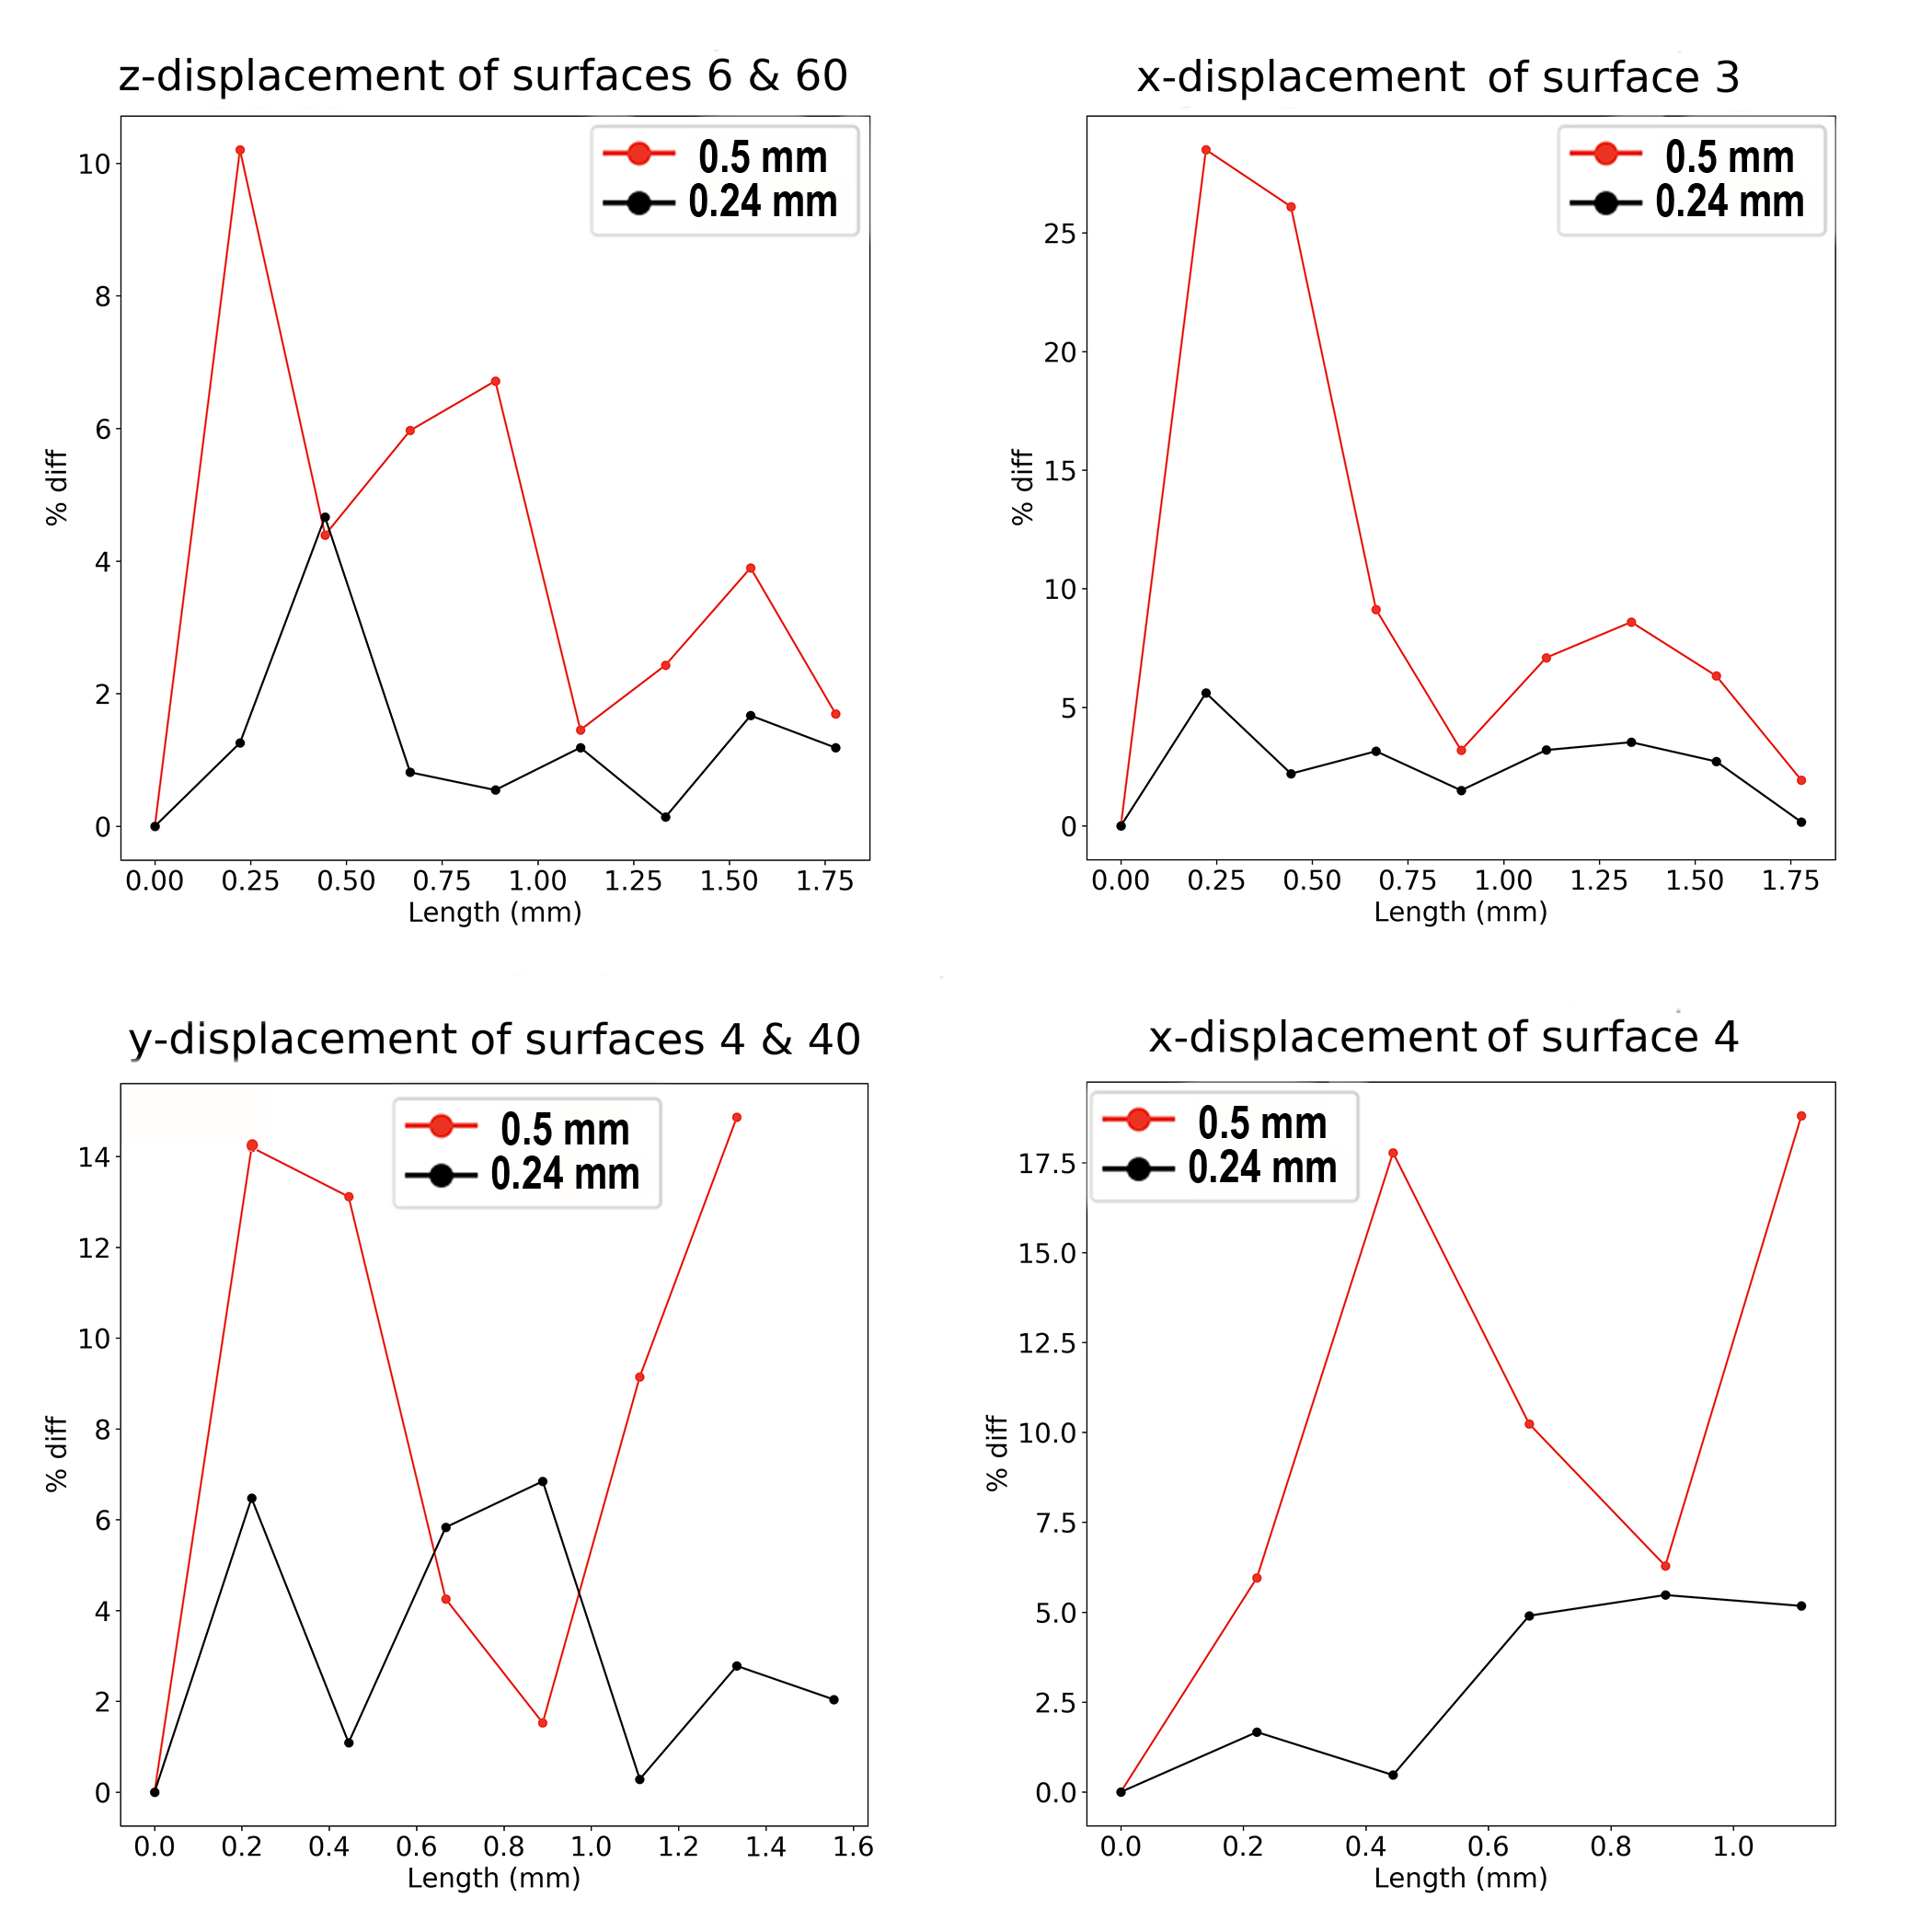
\includegraphics[width=\textwidth,height=\textheight,keepaspectratio]{crack_convergence.png}
\caption{Convergence of crack growth step size for each of the four different
displacement boundary conditions. The percent difference is calculated with respect
to a 0.15 mm crack growth step size.
}
\label{fig:crack_convergence}
\end{figure}

\begin{figure}[h!]
  \begin{subfigure}[b]{0.5\textwidth}
    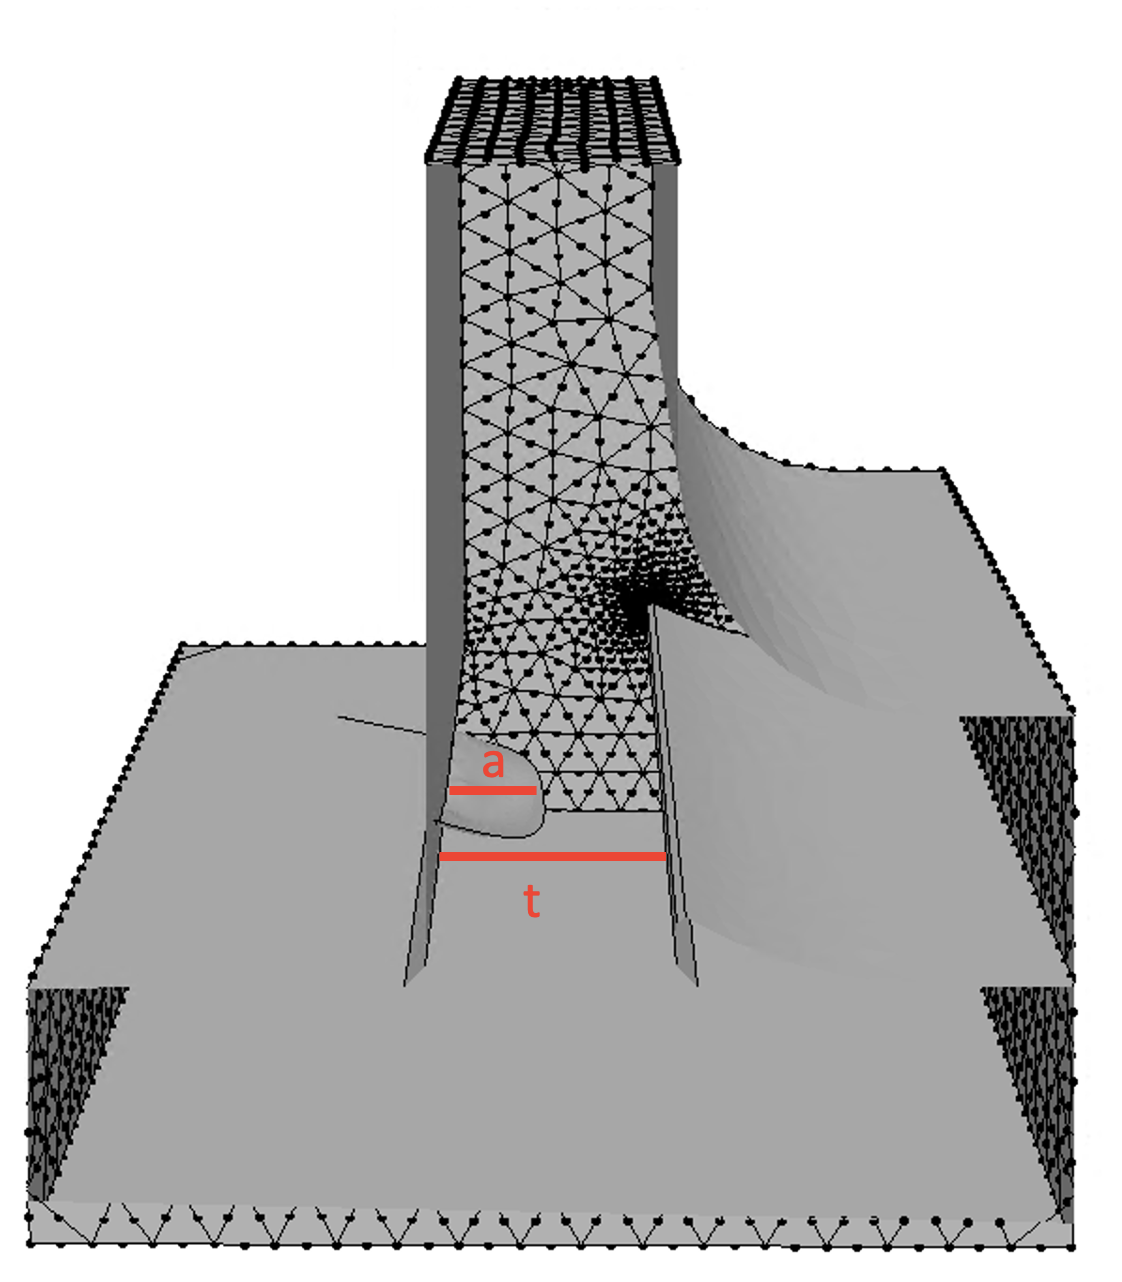
\includegraphics[width=\textwidth]{horizontal_growth.png}
    \caption{Horizontal growth path}
    \label{fig:horizontal_growth}
  \end{subfigure}
  \hfill
  \begin{subfigure}[b]{0.5\textwidth}
    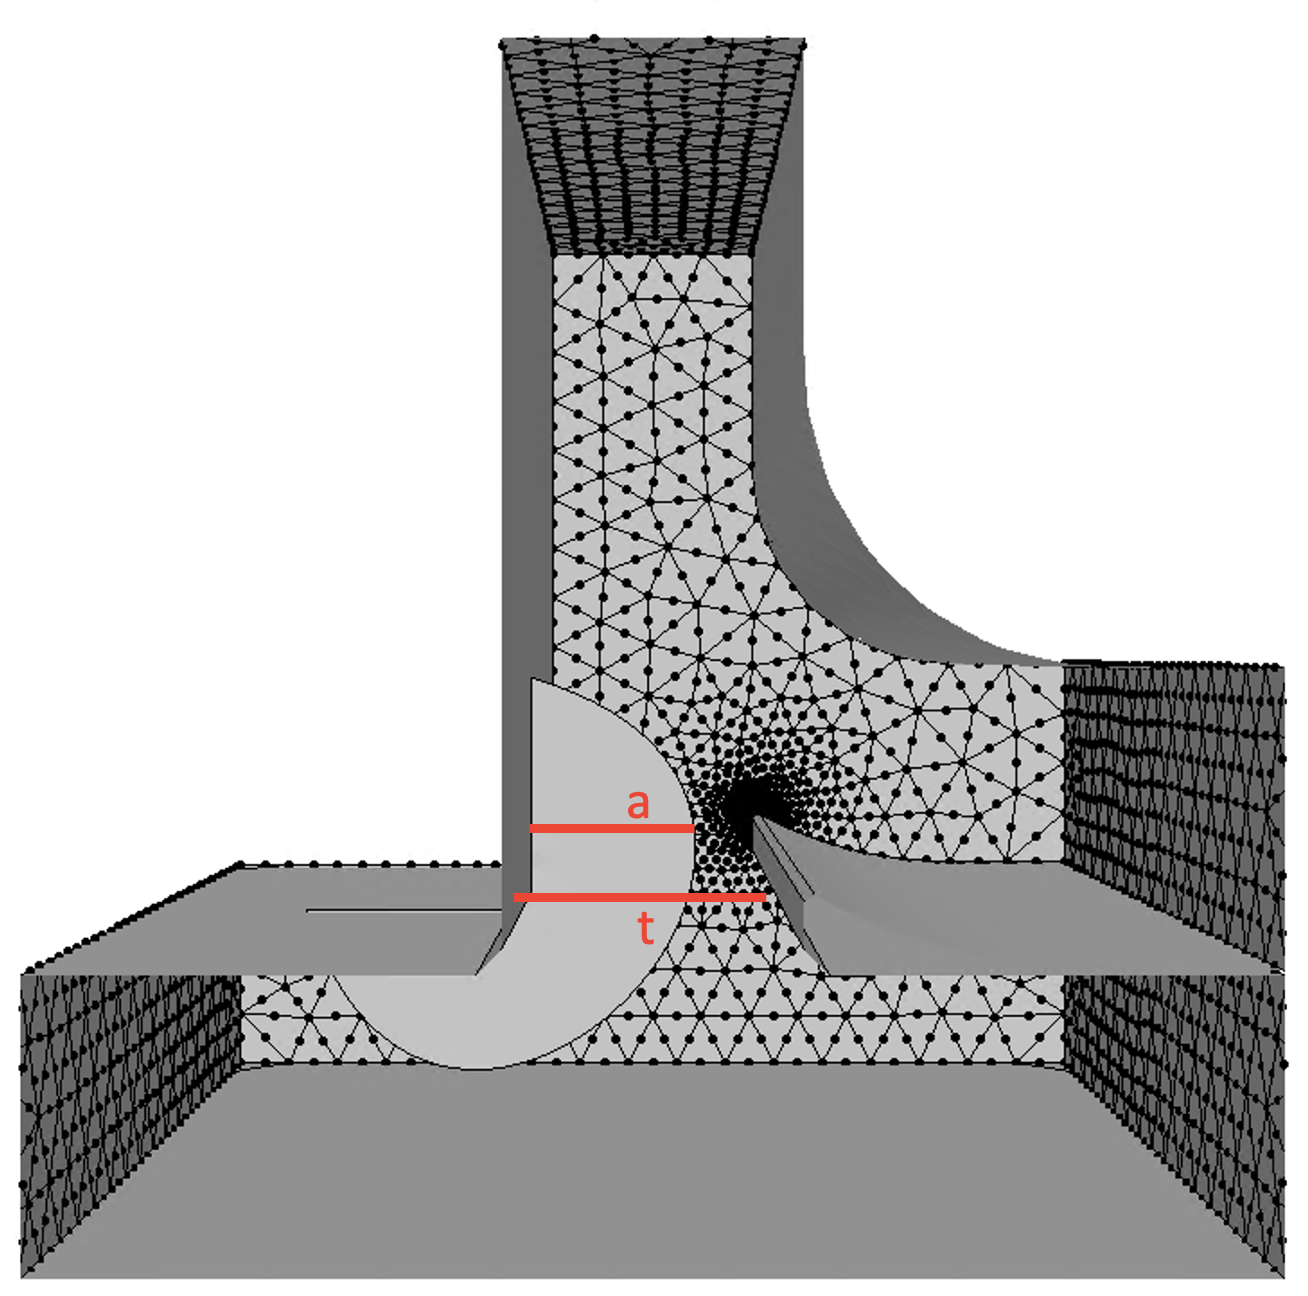
\includegraphics[width=\textwidth]{horizontal_growth2.png}
    \caption{Horizontal growth path}
    \label{fig:horizontal_growth2}
  \end{subfigure}
  \hfill
  \begin{subfigure}[b]{0.5\textwidth}
    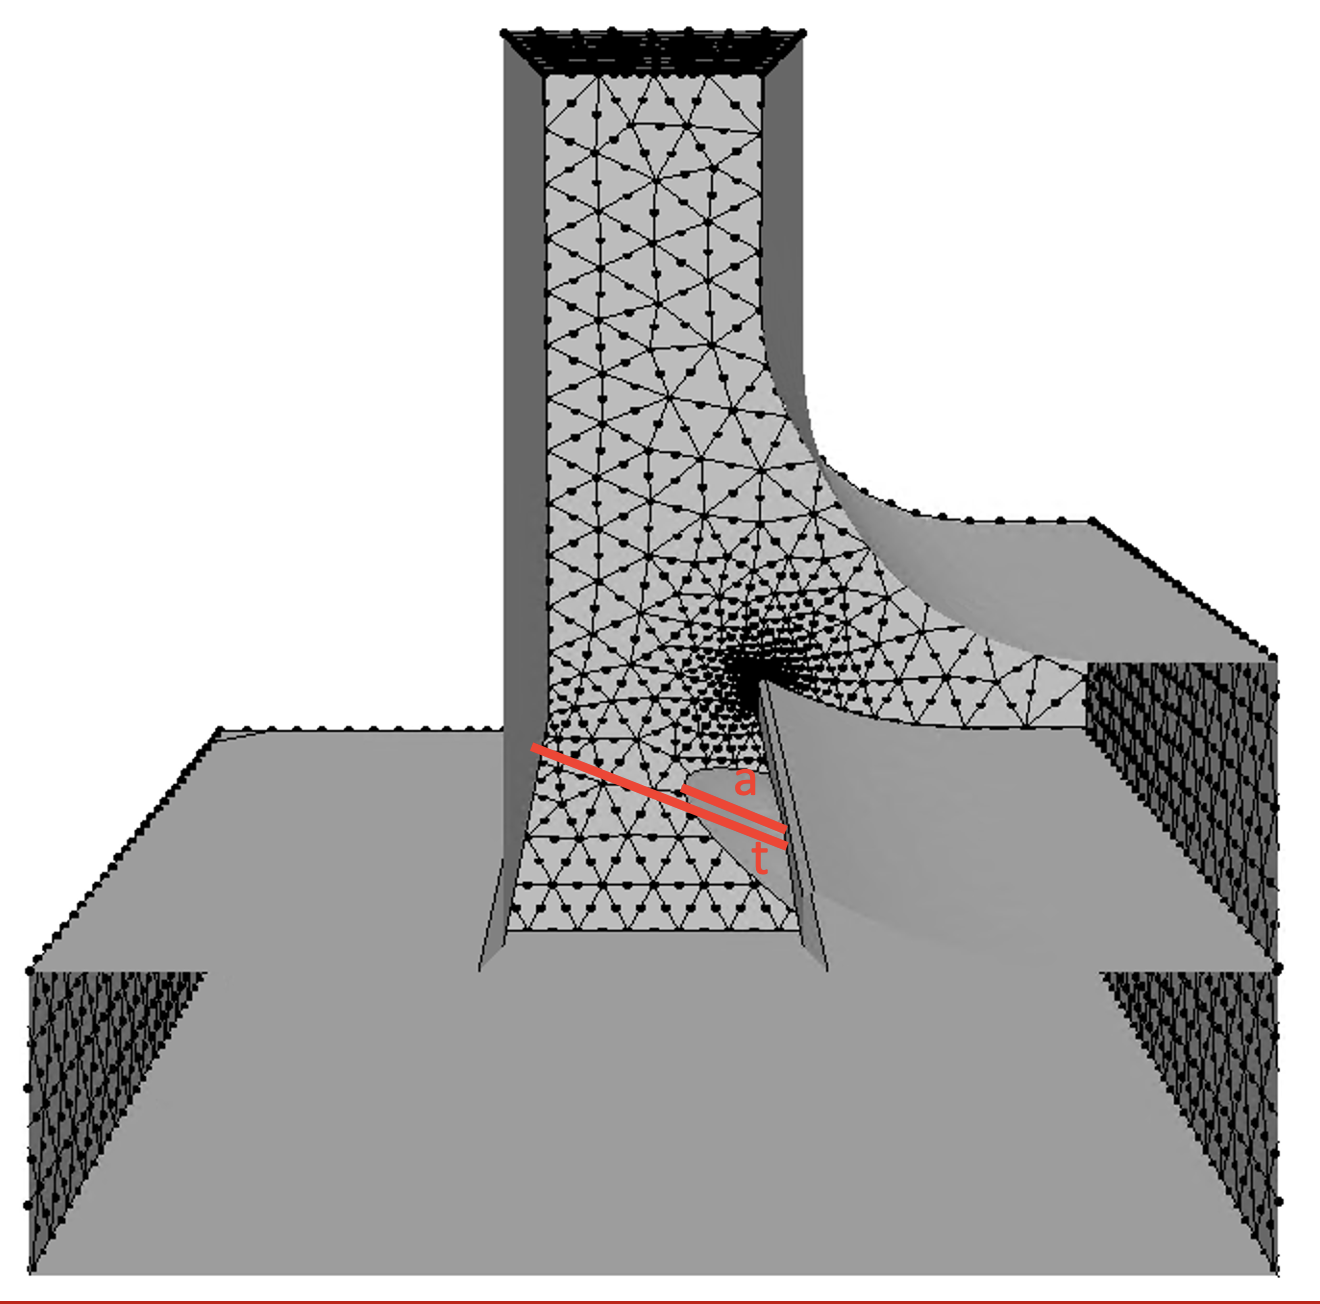
\includegraphics[width=\textwidth]{upward_growth.png}
    \caption{Horizontal upward growth path}
    \label{fig:upward_growth}
  \end{subfigure}
  \hfill
  \begin{subfigure}[b]{0.5\textwidth}
    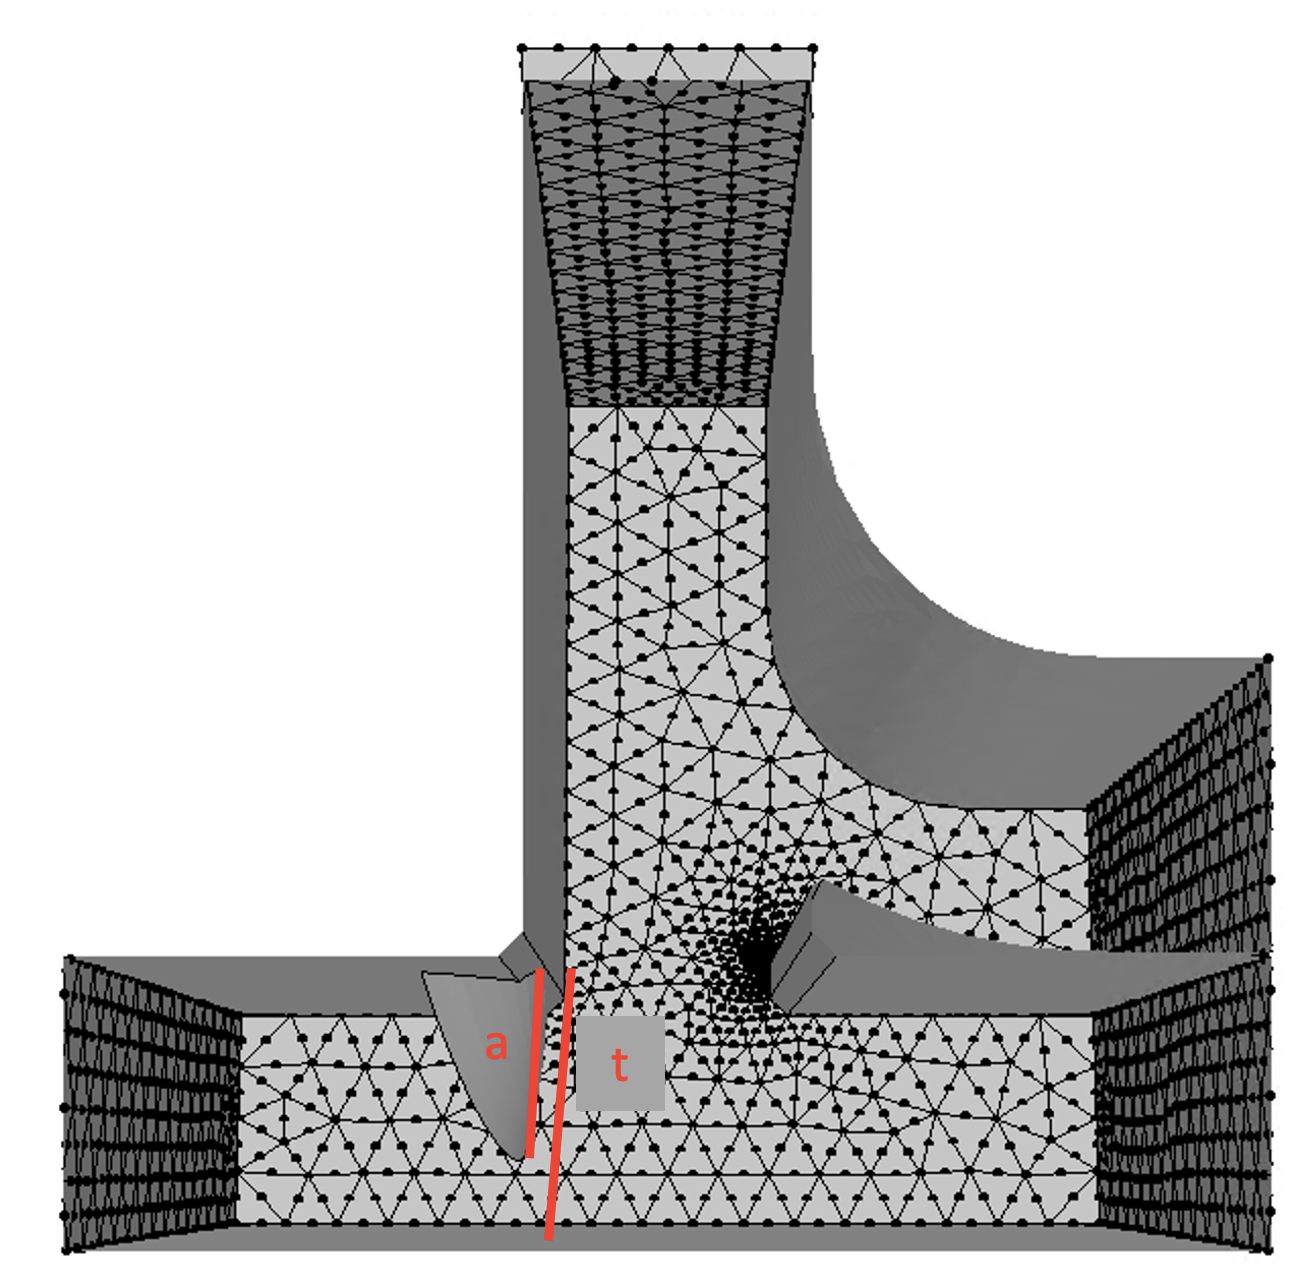
\includegraphics[width=\textwidth]{downward_growth.png}
    \caption{Downward growth}
    \label{fig:downward_growth}
  \end{subfigure}
  \caption{Four examples illustrating the variety of different growth paths the
cracks followed. Each figure shows how both the crack depth $a$ and the thickness
$t$ were defined in the different cases.}
  \label{fig:crack_paths}
\end{figure}

\begin{figure}[h!]
\centering
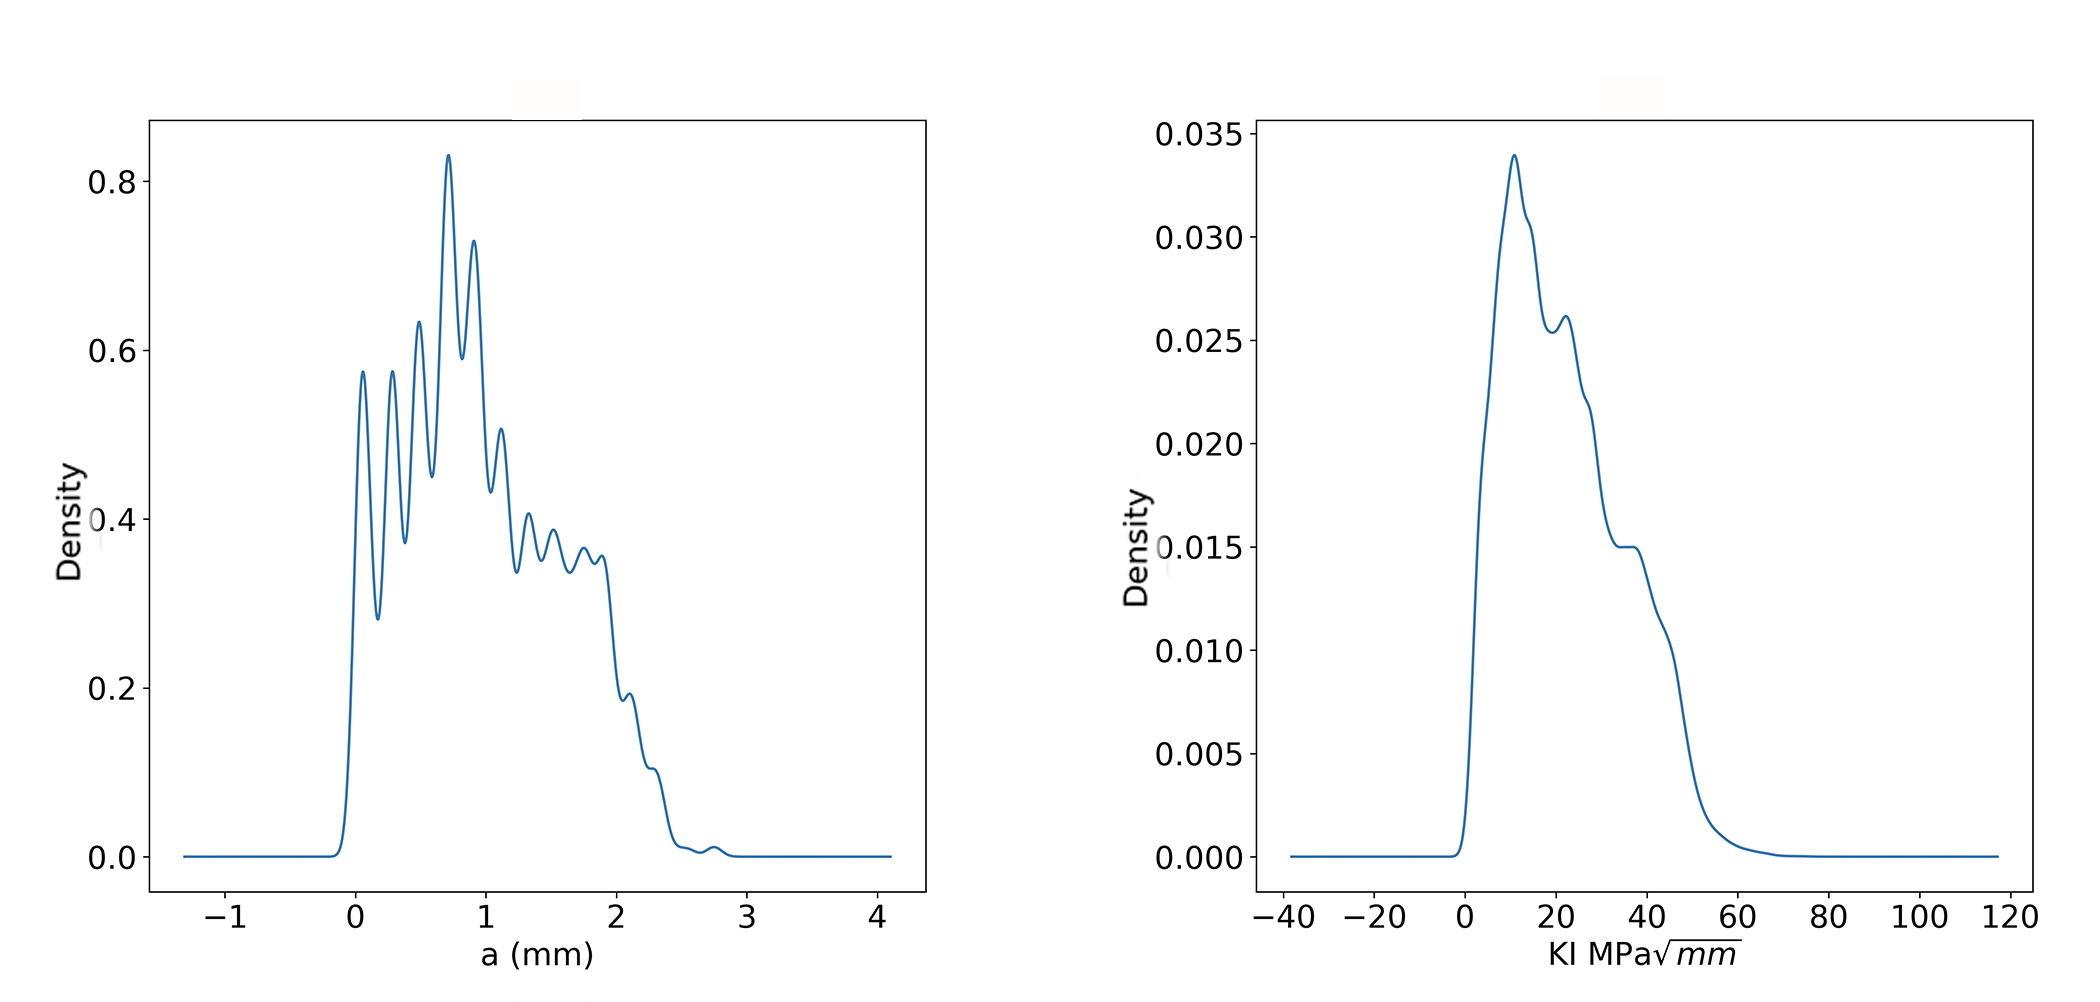
\includegraphics[width=\textwidth,height=300pt,keepaspectratio]{aKI_pde.png}
\caption{Density curves of two of the variables calculated as a result of
computational fracture analysis. Crack depth, a, and $K_I$.
}
\label{fig:aKI_pde}
\end{figure}

\begin{figure}[h!]
\centering
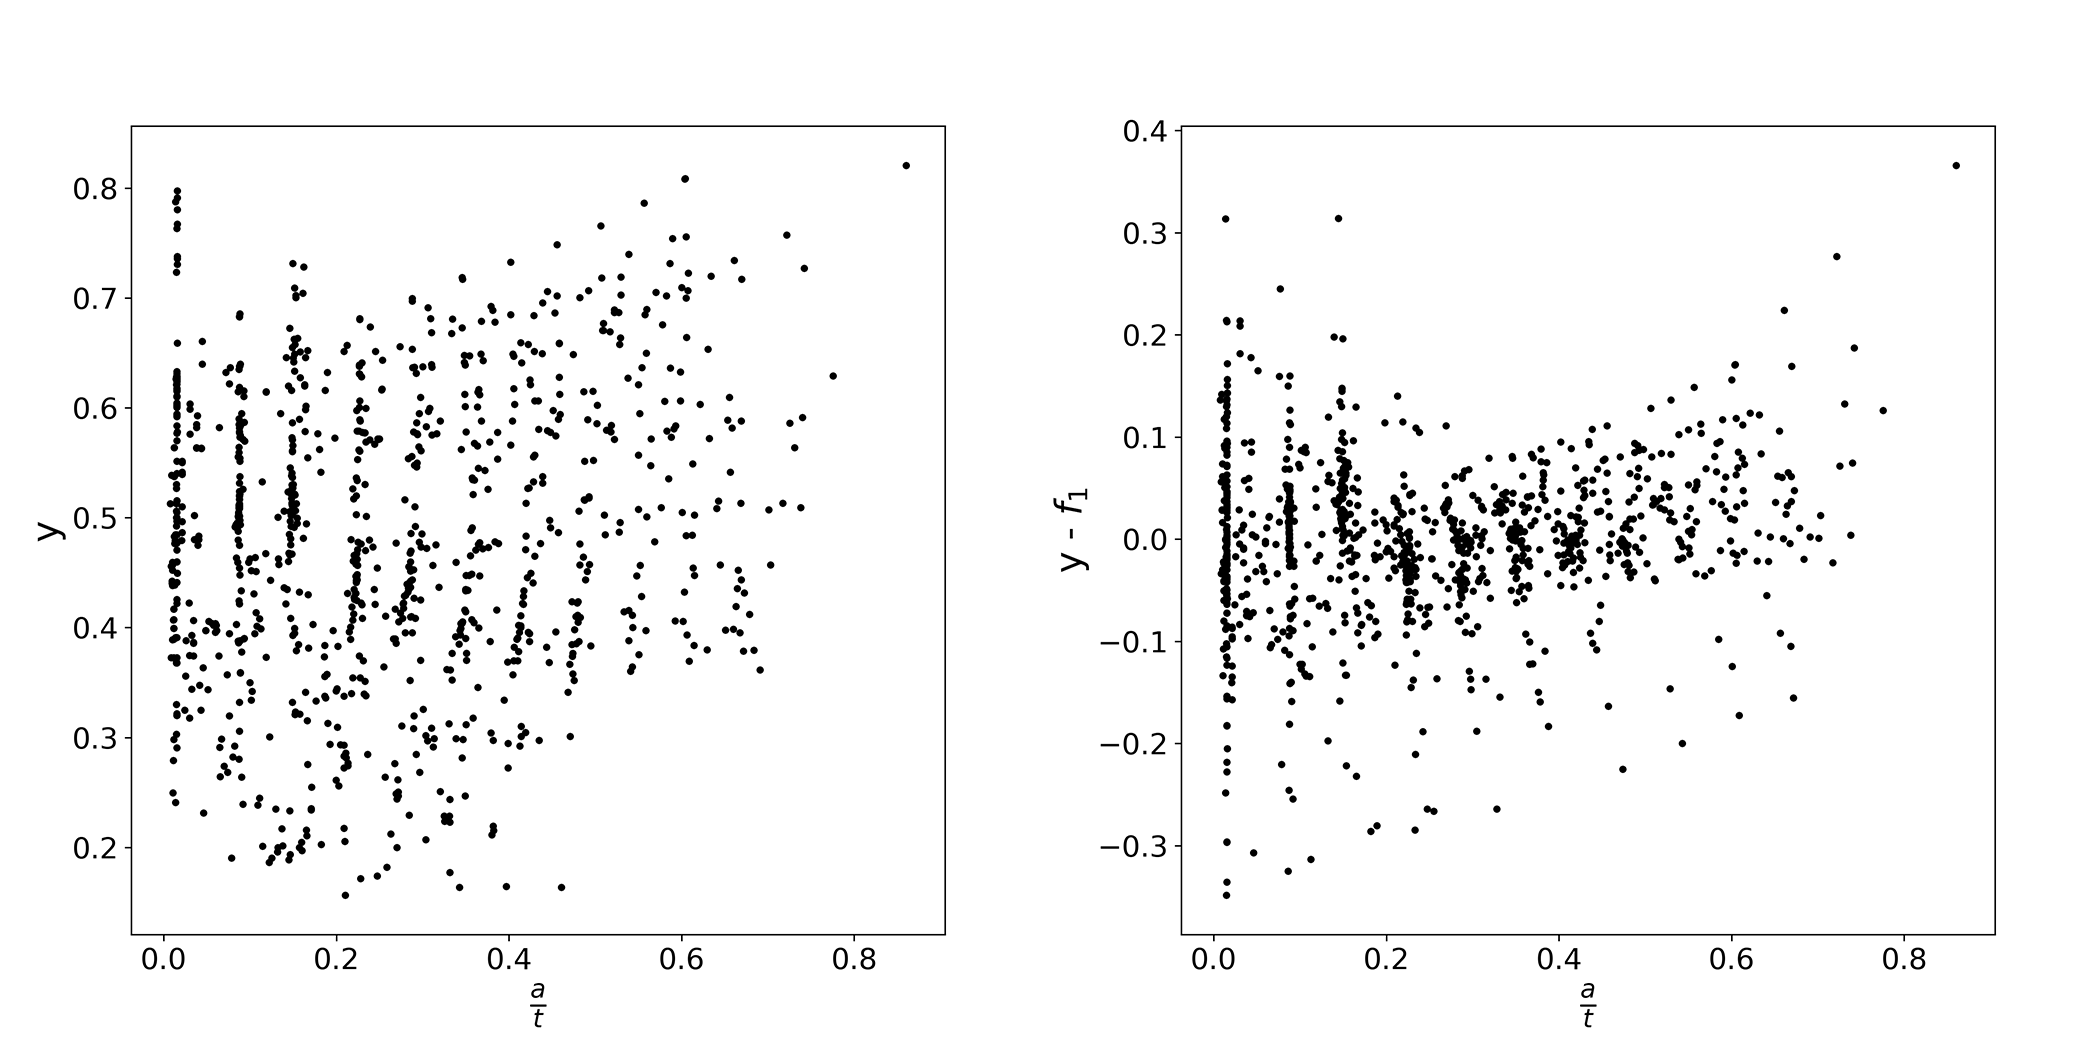
\includegraphics[width=\textwidth,height=300pt,keepaspectratio]{f_fsubm1.png}

\caption{Plots for the ground truth with respect to $\frac{a}{t}$ and the ground
truth subtracted by the first model with respect to $\frac{a}{t}$. Showing high
amounts of scatter in the ground truth.  }

\label{fig:f_fsubm1}
\end{figure}

\begin{figure}[h!]
\centering
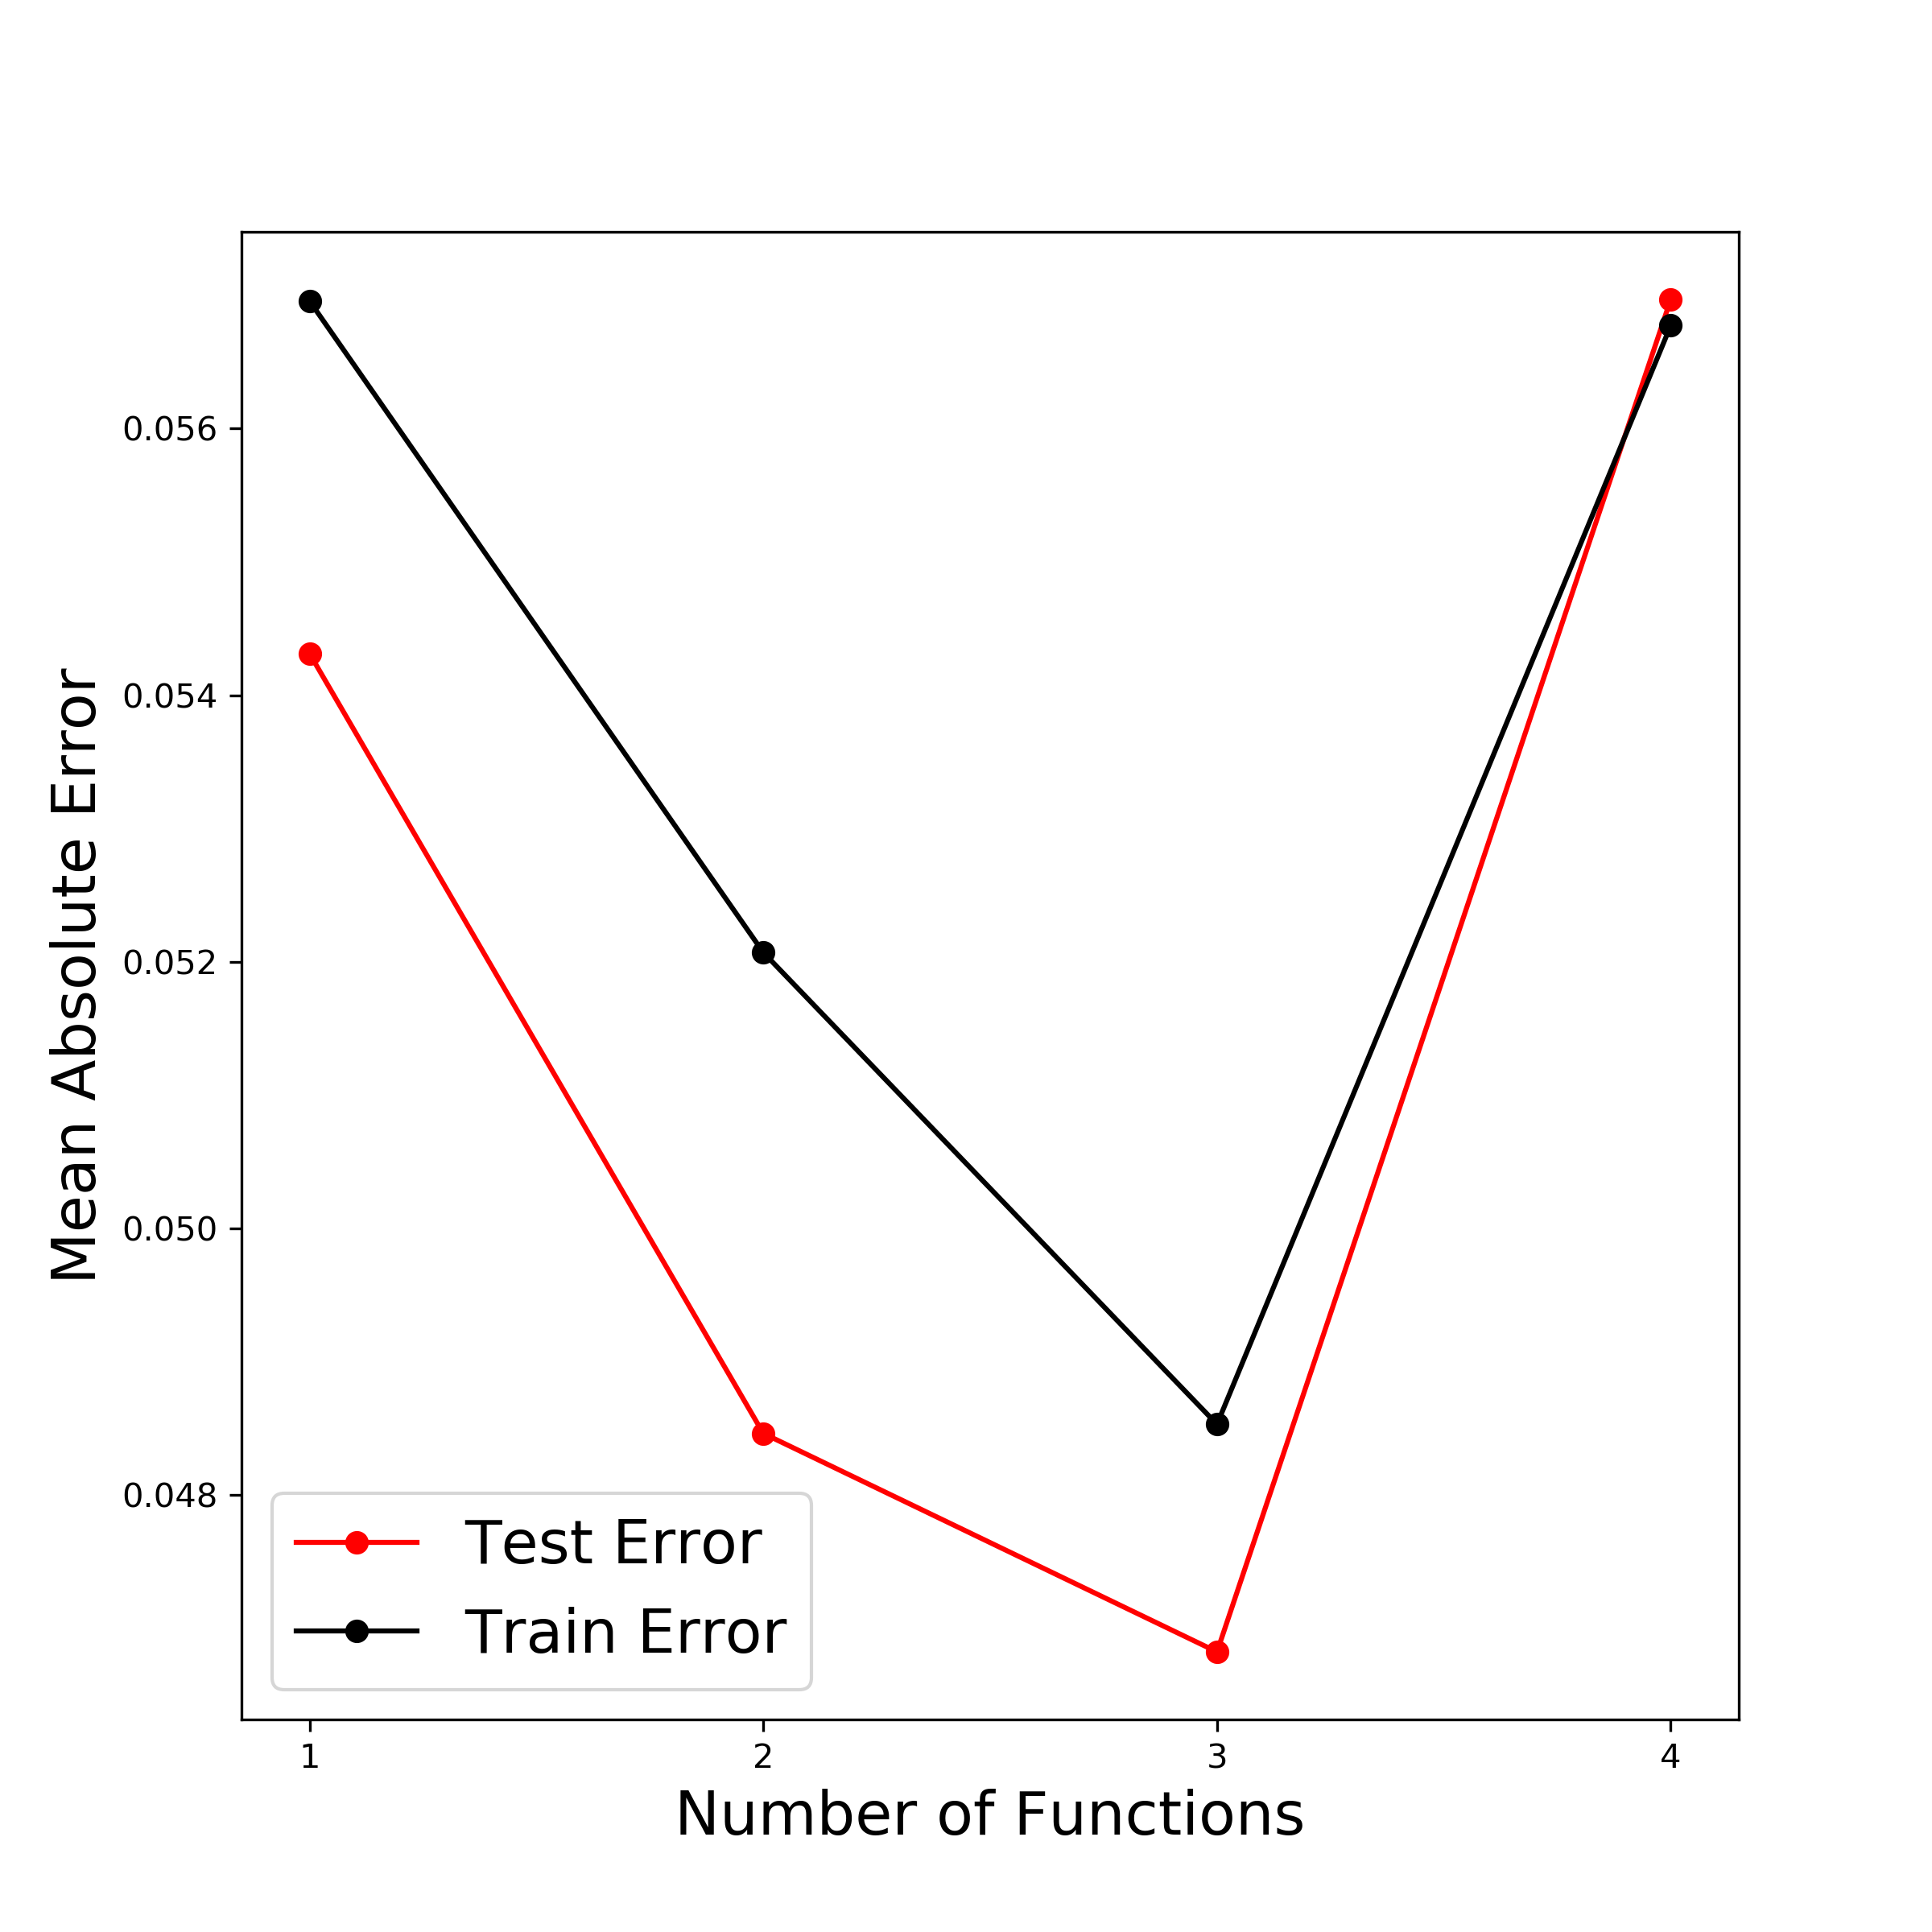
\includegraphics[width=\textwidth,height=300pt,keepaspectratio]{models_performance.png}

\caption{Mean absolute error of the training data and the test data with the
addition of more models.}
\label{fig:models_performance}
\end{figure}

\begin{figure}[h!]
  \begin{subfigure}[b]{0.5\textwidth}
    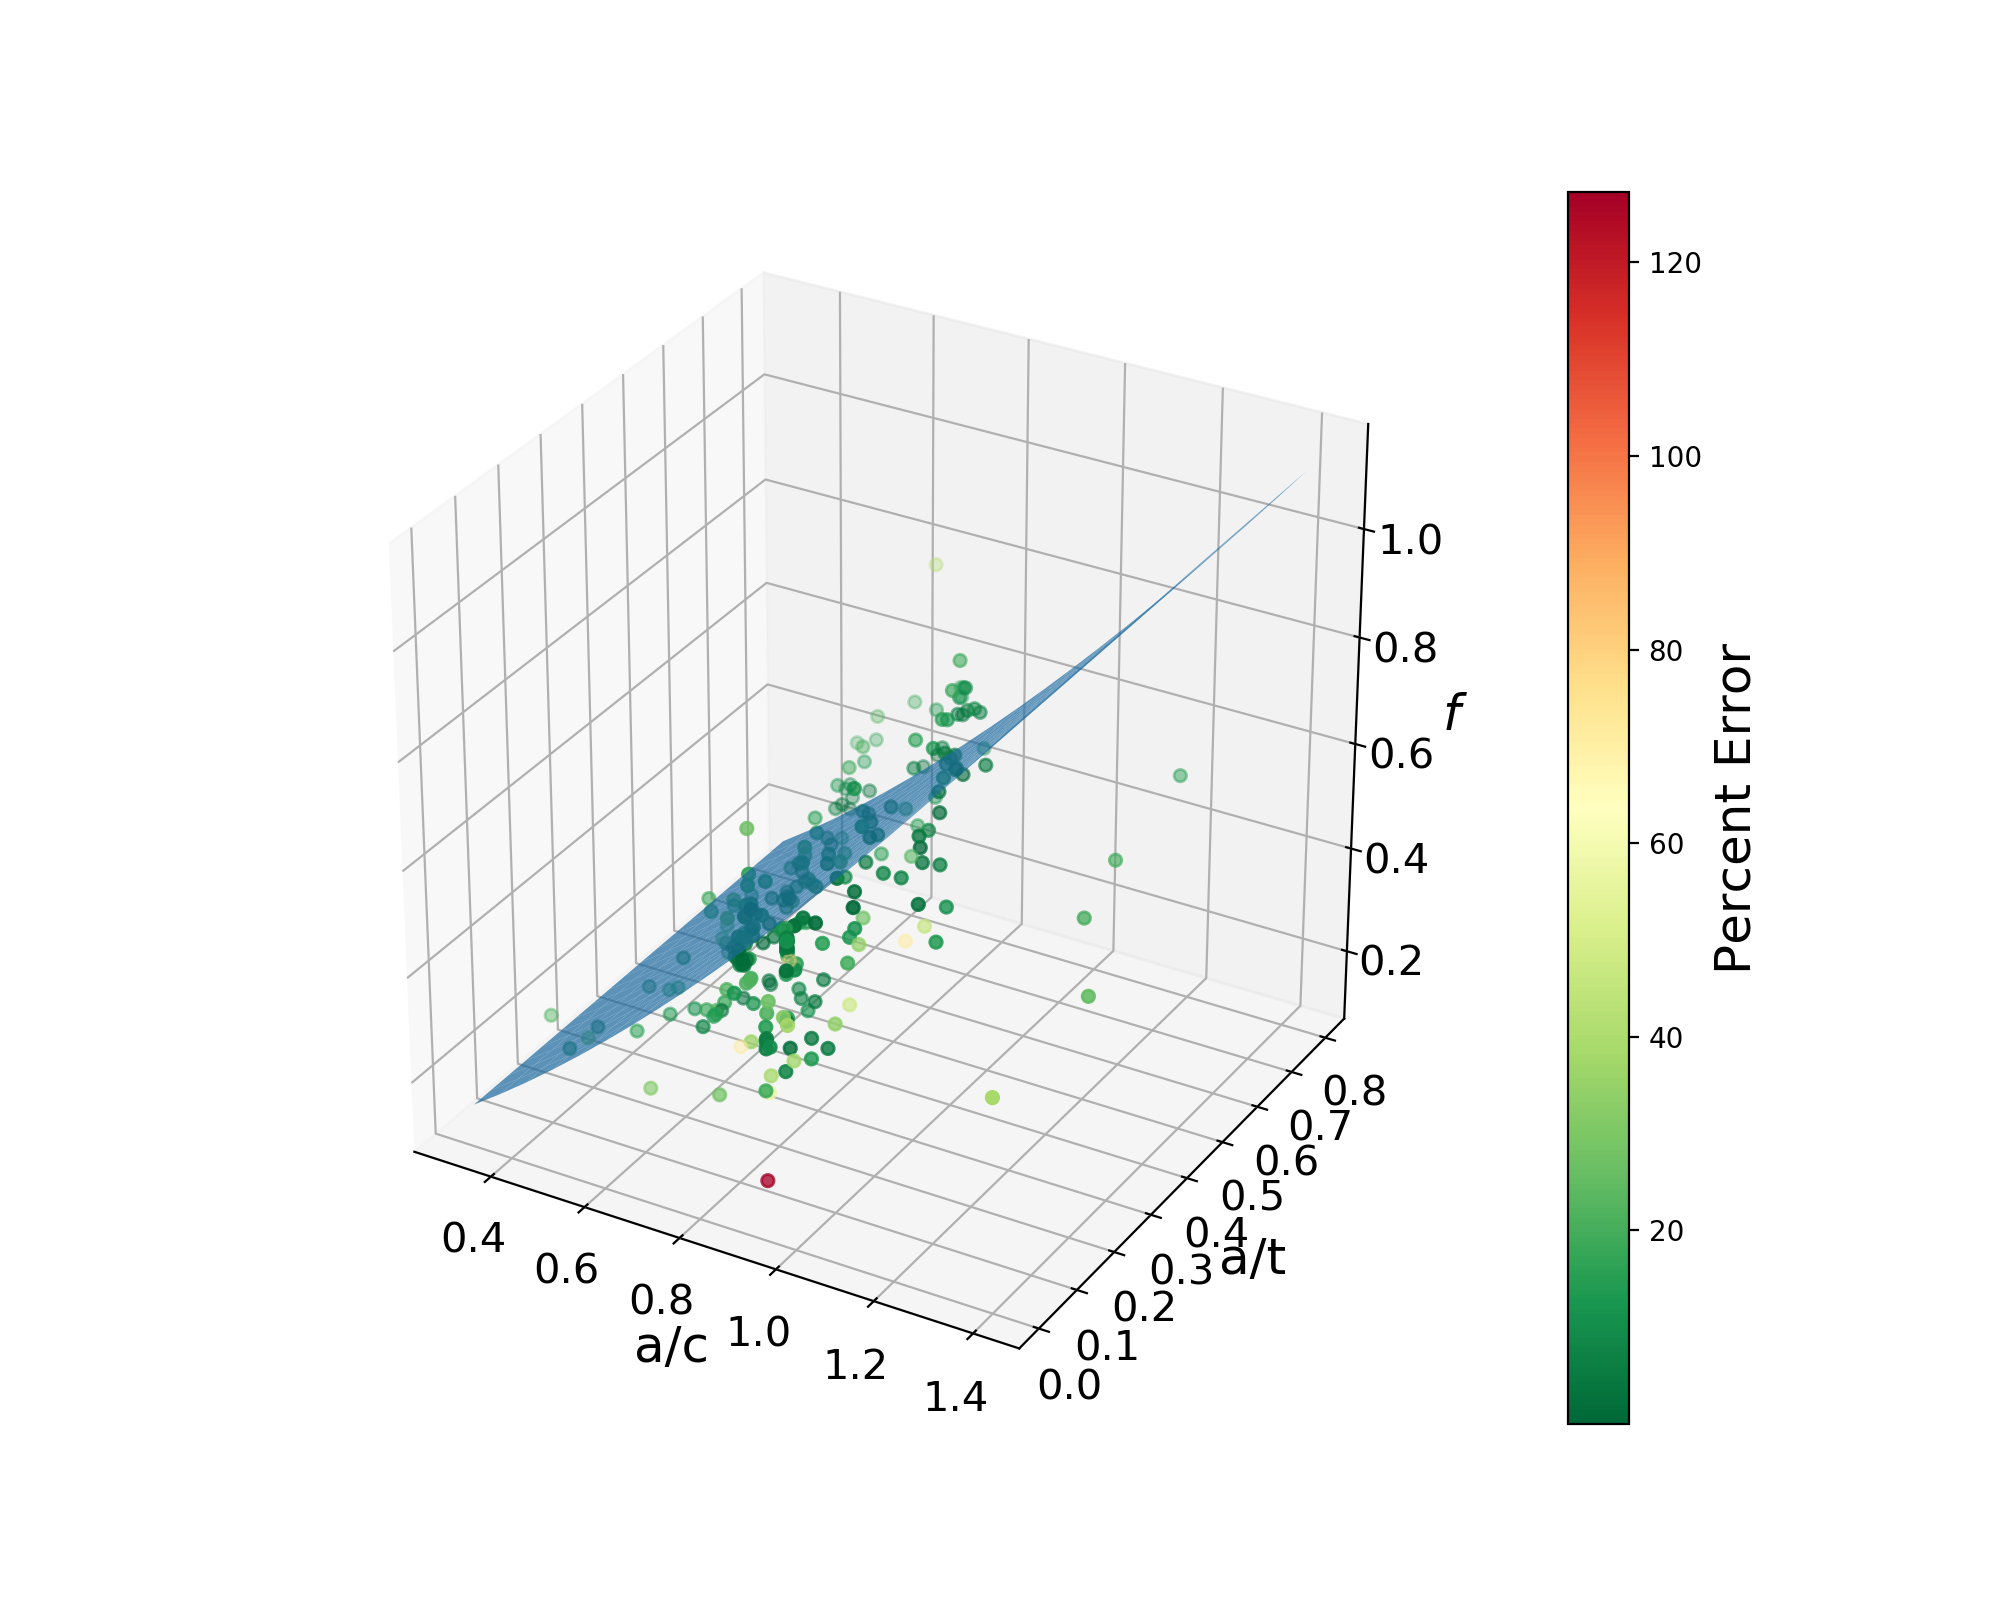
\includegraphics[width=\textwidth]{f1_surf.png}
    \caption{$f_1$ compared to the data}
    \label{fig:f1_surf}
  \end{subfigure}
  \hfill
  \begin{subfigure}[b]{0.5\textwidth}
    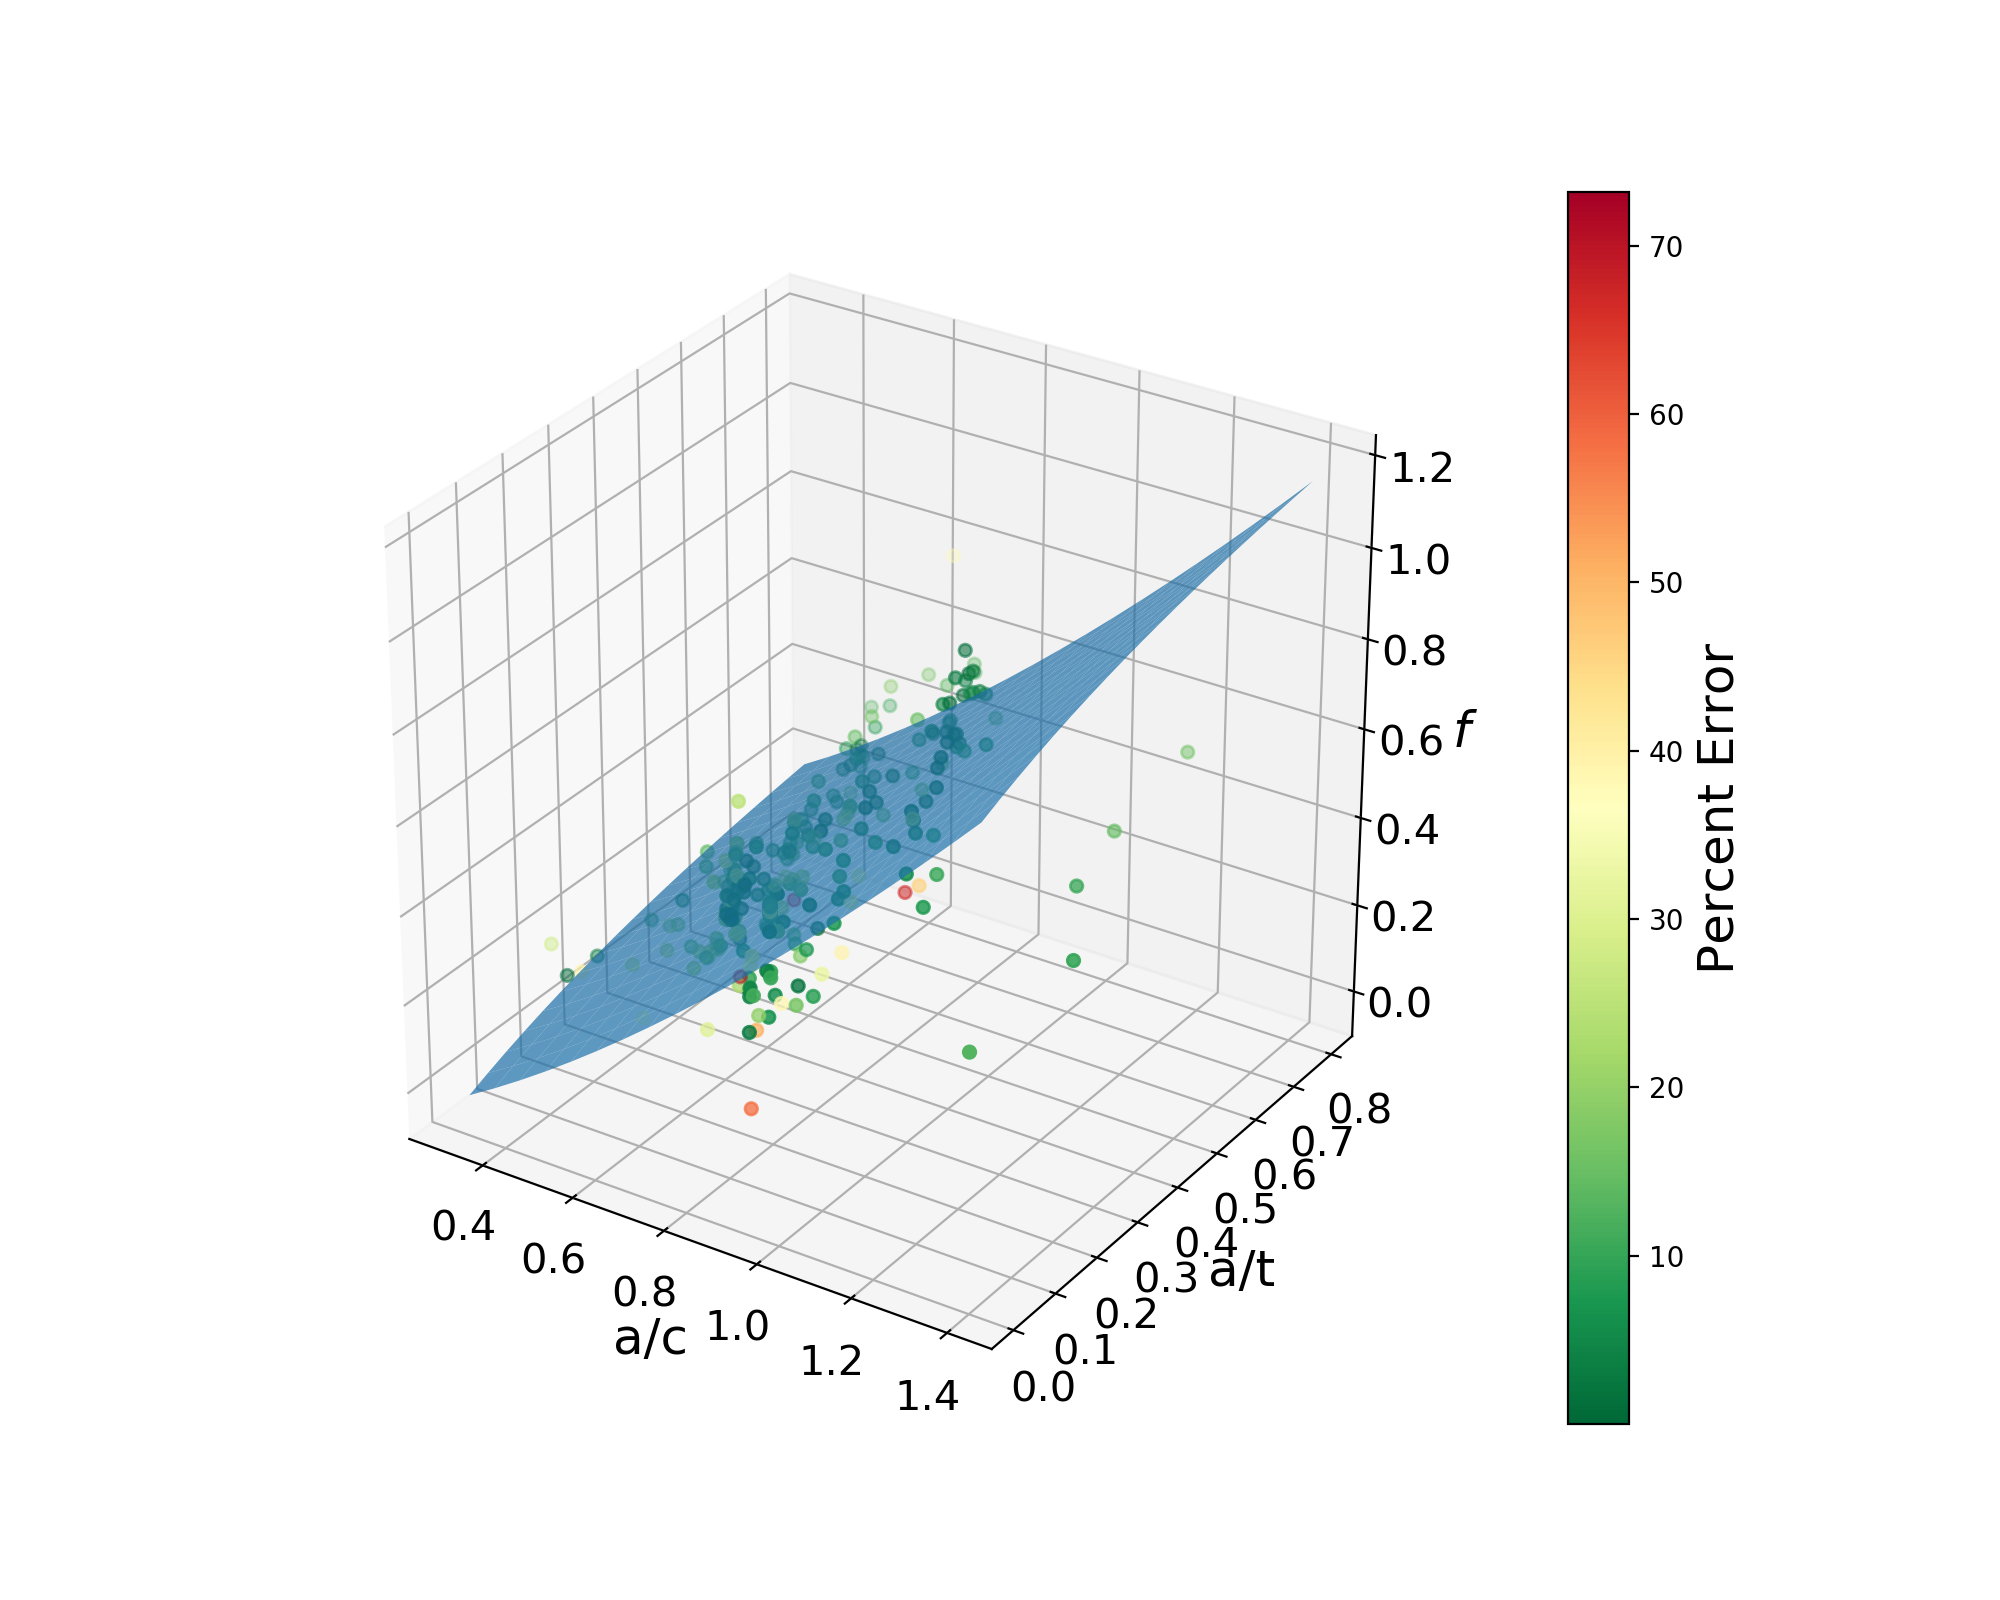
\includegraphics[width=\textwidth]{f1f2_surf.png}
    \caption{$f_1 + f^{'}_{2}$ compared to the data}
    \label{fig:f2_surf}
  \end{subfigure}
  \hfill
  \begin{subfigure}[b]{0.5\textwidth}
    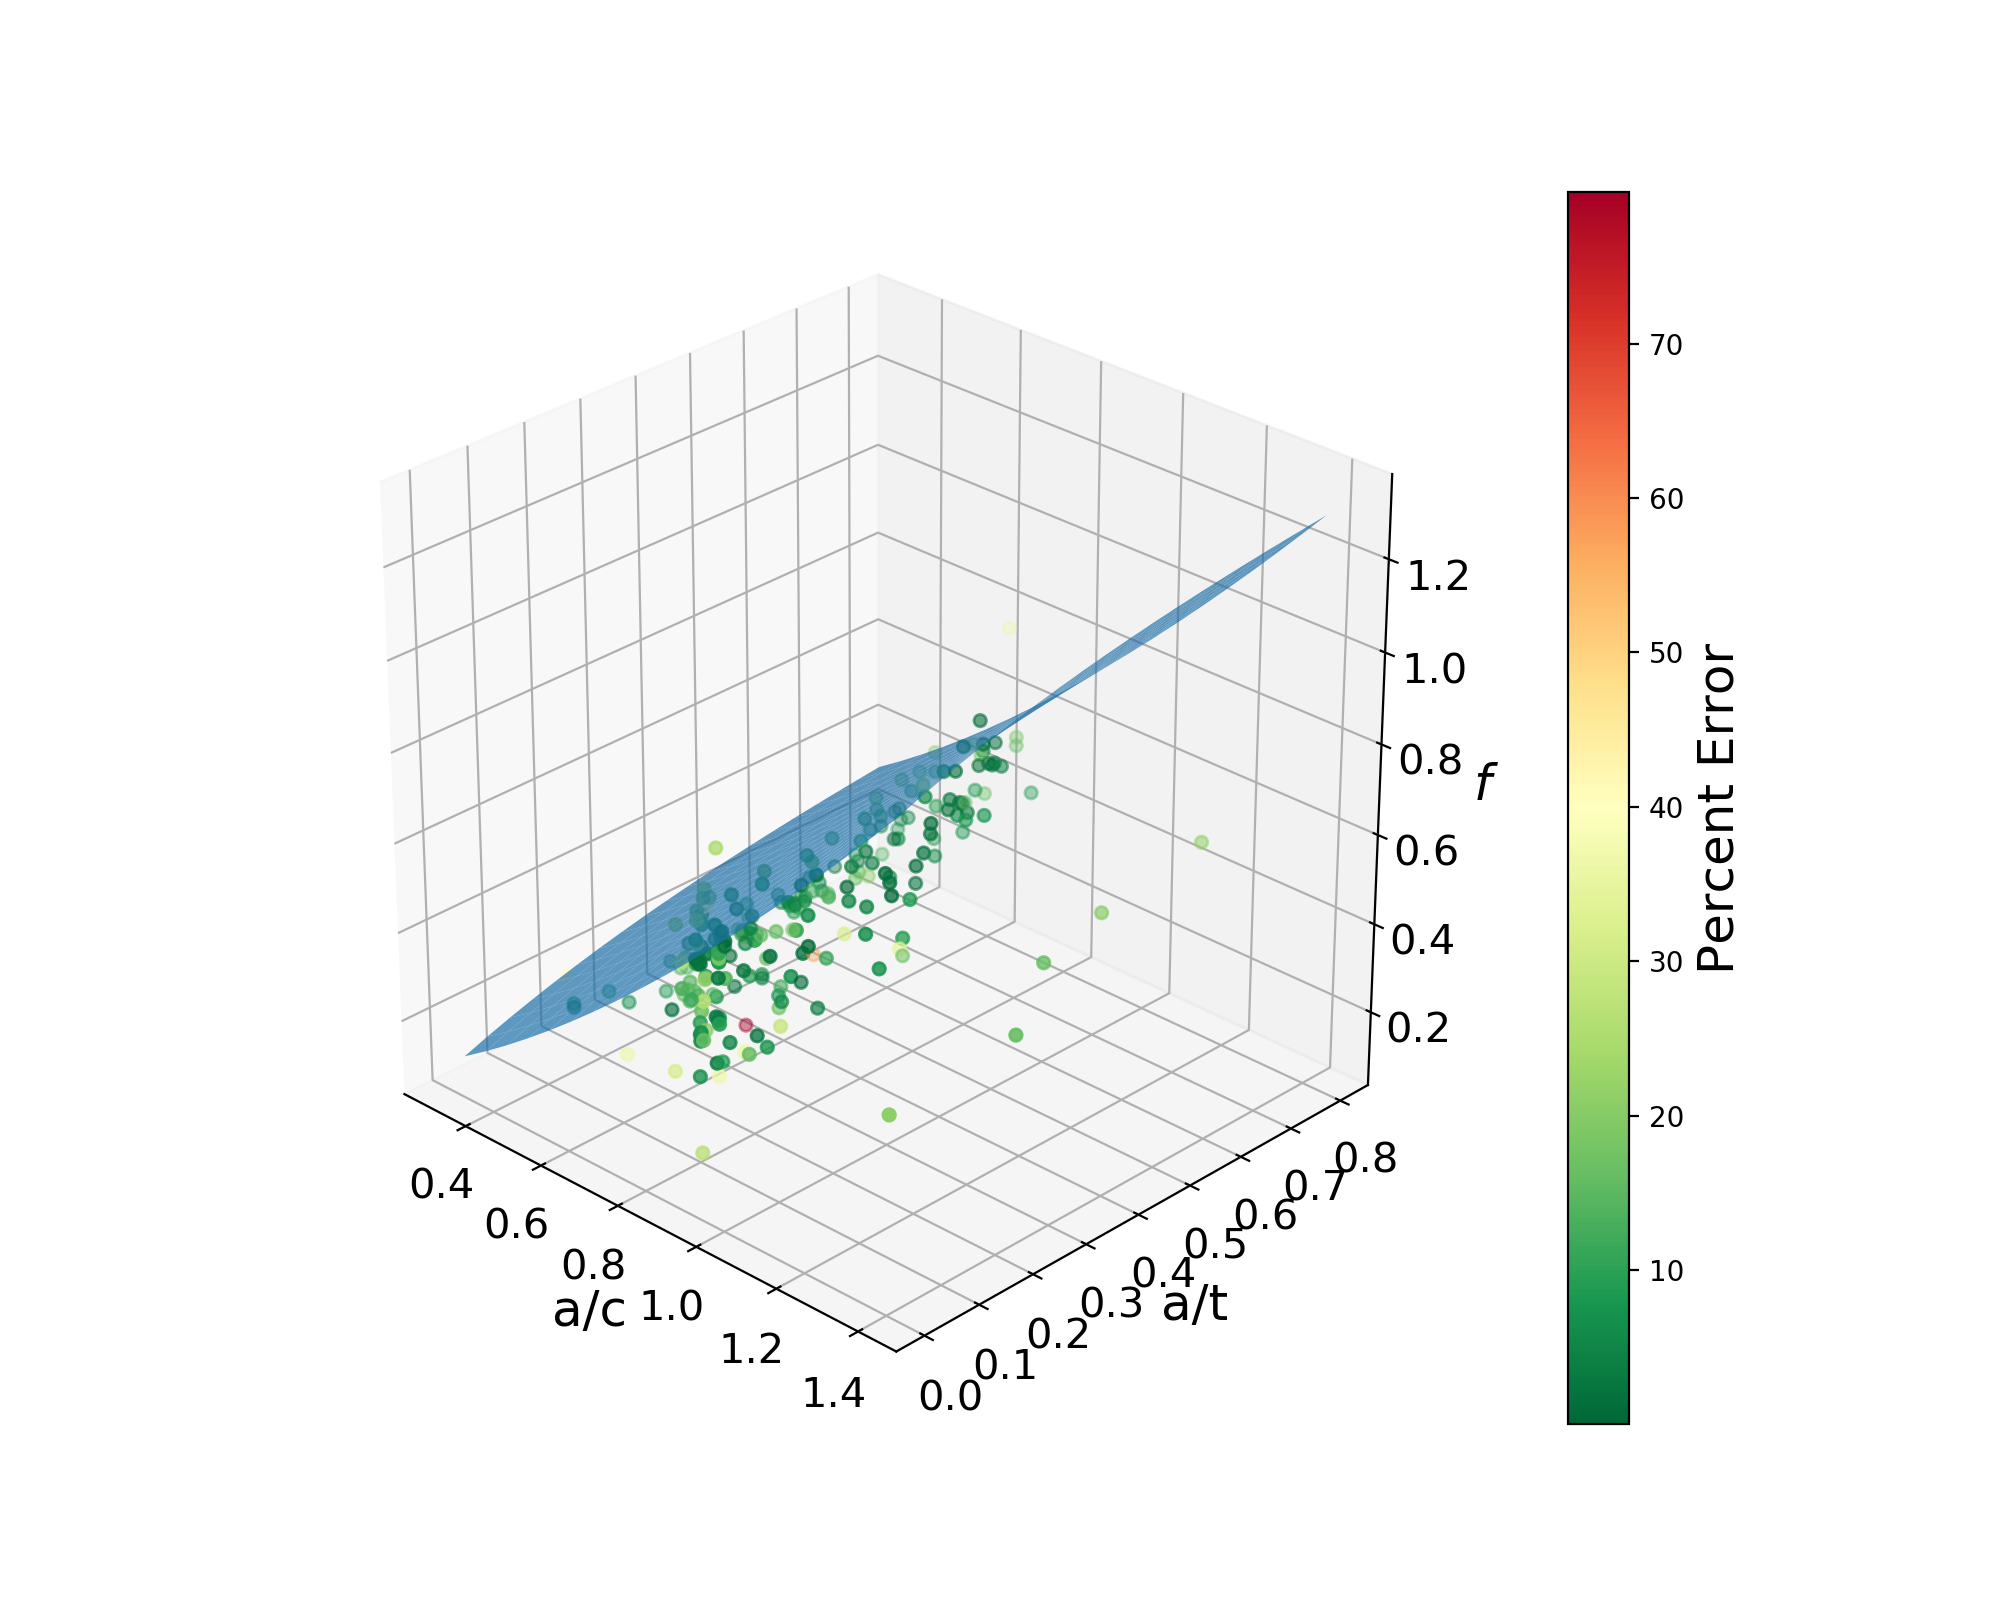
\includegraphics[width=\textwidth]{f1f2f3_surf.png}
    \caption{$f_1 + f^{'}_{2} + f_3$ compared to the data}
    \label{fig:f3_surf}
  \end{subfigure}
  \hfill
  \begin{subfigure}[b]{0.5\textwidth}
    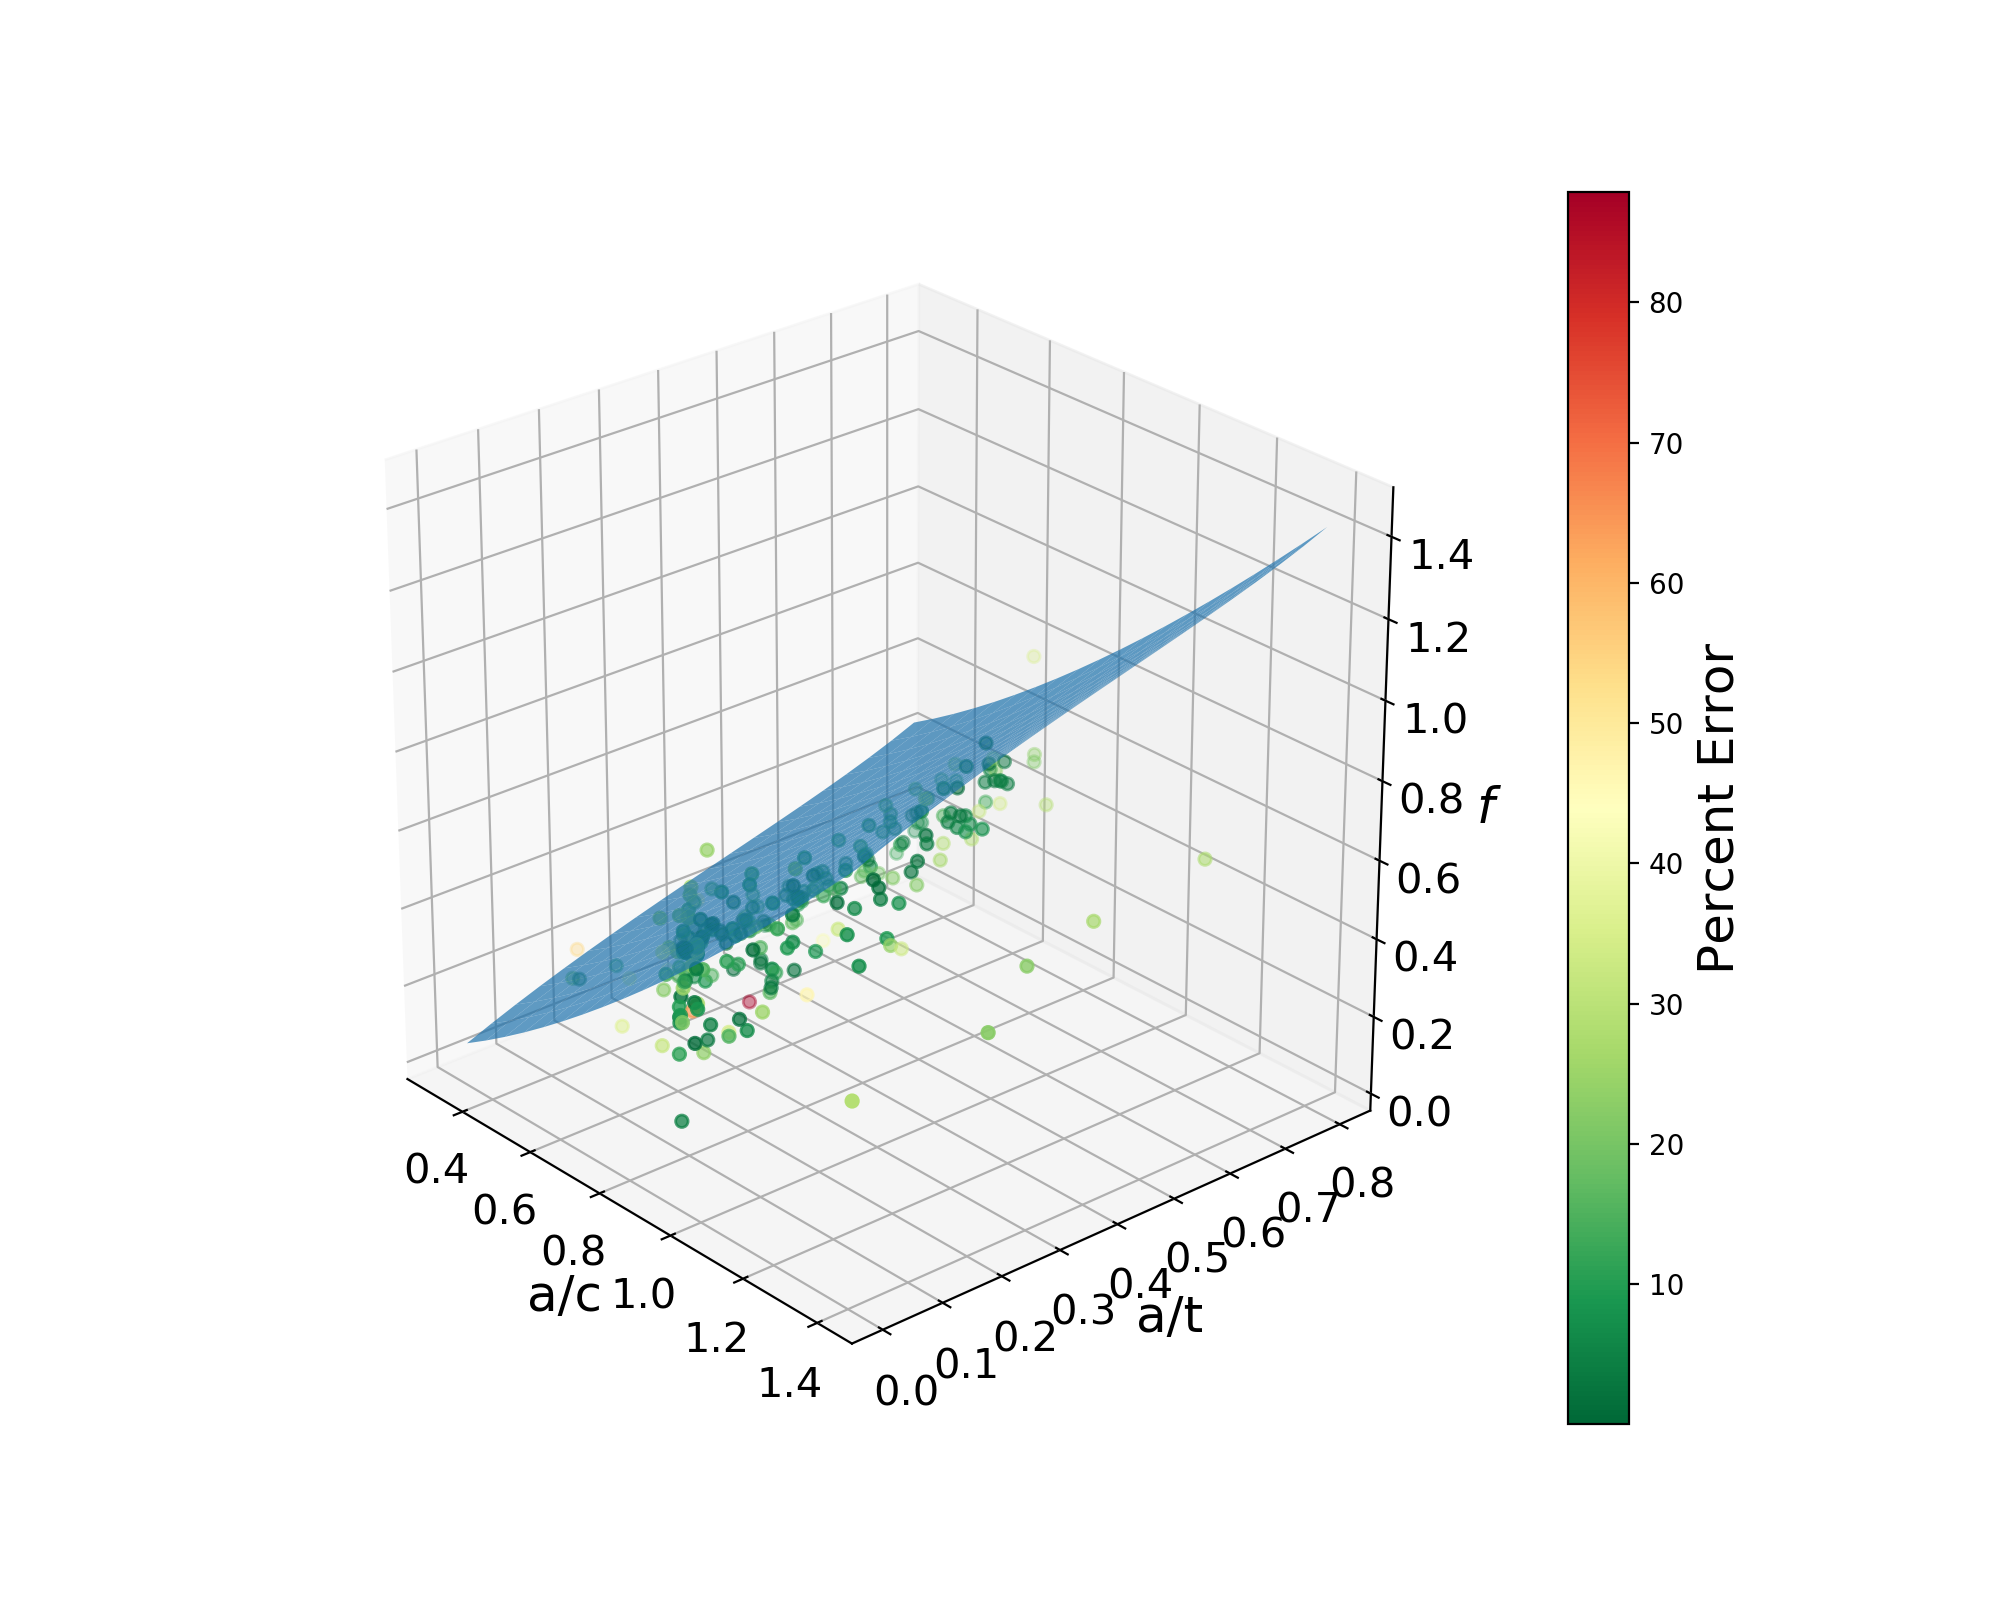
\includegraphics[width=\textwidth]{f1f2f3f4_surf.png}
    \caption{$f_1 + f^{'}_{2} + f_3 + f_4$ compared to the data}
    \label{fig:f4_surf}
  \end{subfigure}

  \caption{Three-dimensional slices of the six-dimensional data with
$\frac{a}{c}$ and $\frac{a}{t}$ as the displayed input variables of $f$ The
surfaces represents the functions.}

\end{figure}

%END OF CHAPTER TABLES

\begin{table}[h!]
\centering
\label{tab:max_disps}
\caption{\label{tab:max_disps}Maximum applied displacements of each boundary
condition such that displacement error between the structural- and solid-element
models remains below 1\%}

\begin{tabular}{ |c|c| } 
\hline
Disp. BC & Maximum displacement (mm) \\
\hline
z-displacement on surfaces 6 \& 60 & 0.03 \\ 
x-displacement on surface 3 & 0.01 \\ 
y-displacement on surfaces 4 \& 40 & 0.02\\ 
x-displacement on surface 4 & 0.03 \\ 
\hline
\end{tabular}
\end{table}

\begin{table}[h!]
\centering
\label{tab:sobol_indices}
\caption{\label{tab:sobol_indices}The first order and total sensitivity index as
defined by Sobol' for each displacement BC and their effect on maximum principal
stress as well as their confidence intervals.}
\begin{tabular}{ |c|c|c|c|c| } 
\hline
Disp. BC & S1 & 95\% CI & ST & 95\% CI \\
\hline
z-displacement on surfaces 6 \& 60 & 0.167 & 0.182 & 0.128 & 0.089 \\ 
x-displacement on surface 3 & 0.0145 & 0.312 & 0.239 & 0.334 \\ 
y-displacement on surfaces 4 \& 40 & 0.203 & 0.257 & 0.189 & 0.162 \\ 
x-displacement on surface 4 & 0.303 & 0.300 & 0.274 & 0.230 \\ 
\hline
\end{tabular}
\end{table}

\begin{table}[h!]
\centering
\label{tab:fitnesses}

\caption{\label{tab:fitnesses}Mean absolute error of each summed model including
the simplified model of $f_2$, $f^{'}_{2}$}

\begin{tabular}{ |c|c| } 
\hline
Summed Models & Mean Absolute Error \\
\hline
$f_1$ & 0.0543 \\ 
$f_1 + f_2$ & 0.0482 \\ 
$f_1 + f_2 + f_3$ & 0.0466 \\
$f_1 + f_2 + f_3 + f_3$ & 0.0570 \\
$f_1 + f^{'}_{2}$ & 0.0485 \\ 
$f_1 + f^{'}_{2} + f_3$ & 0.0468 \\
$f_1 + f^{'}_{2} + f_3 + f_3$ & 0.0570 \\
\hline
\end{tabular}
\end{table}
%%% -*-LaTeX-*-

\chapter{Conclusion}\label{conclusion}

A surrogate model for crack growth through a weld is obtained using symbolic regression. The surrogate model inputs are: crack geometry, crack orientation, and growth angle. The data was collected from 180 different boundary condition configurations of a model. For each boundary condition configuration, a crack is grown in the model through the weld in the least conservative location and orientation. 

The resulting surrogate model is a symbolic equation from which we can interpret the effect of each input variable on the prediction of stress intensity factors. The final model is a summation of multiple equations that resulted from using a gradient boosting technique. It has been shown that the application of gradient boosting in symbolic regression can yield models with lower error without over-fitting to the training data. 

We were unable to find a surrogate model to map the stresses in the shell element line welds to the maximum principal stress and the direction of the maximum principal stress. That is left for continuation of the model development. Finding the maximum principal stress from the local line weld stresses will allow the prediction of crack growth using only information gained from shell element simulations. With the current model, assumptions must be made about the stress and crack orientation in order to make a SIF prediction.

Other future work that this project may include is the use of symbolic regression for a more simple, general case. The lessons learned from using symbolic regression on a complicated geometry could be very beneficial to finding a surrogate model for a simple welded plate for example. Other future work may result in different inputs to include in the model that may improve the performance of the models. 

\bibliography{mybibfile}

\end{document}